\documentclass[11pt, a4paper]{article}
\usepackage[utf8]{inputenc}
\usepackage{geometry}
\geometry{margin=1in}
\usepackage{graphicx}
\usepackage{amsmath}
\usepackage{amssymb}
\usepackage{booktabs}
\usepackage{hyperref}
\usepackage{parskip}
\usepackage{array}
\usepackage{longtable}
\usepackage{multirow}
\usepackage{xcolor}
\usepackage{caption}
\usepackage{subcaption}
\usepackage{enumitem}
\usepackage{mathtools}
\usepackage{float}

\hypersetup{
    colorlinks=true,
    linkcolor=blue!70!black,
    citecolor=green!50!black,
    urlcolor=blue!70!black
}

\title{\textbf{Opinion Network Formation: \\ Bipartite ``Extremes'' Sub-Report}}
\author{Tanush Garg \\ IIIT Hyderabad \\ DPCN Assignment 1}
\date{September 2026}

\begin{document}

\maketitle
\tableofcontents
\newpage

%% ─────────────────────────────────────────────────────────────────
\section{Dataset Documentation: Interpretation and Preparation}
%% ─────────────────────────────────────────────────────────────────

The raw dataset comprises survey responses evaluating opinions across four primary thematic domains: \textbf{Technology} (T01--T15), \textbf{Education} (E01--E15), \textbf{Ethics \& Society} (S01--S15), and \textbf{Environment} (V01--V15). The dataset contains \textbf{96 individual respondents} and \textbf{60 distinct questions}, yielding a theoretical maximum of 5,760 individual response data points. After removing 7 respondents with no valid extreme responses, the active network comprises \textbf{89 students} and \textbf{60 questions}.

\subsection{Data Mapping and Ingestion}

The text-based Likert responses were first mapped to a discrete numerical scale to facilitate algorithmic processing:

\begin{center}
\begin{tabular}{clc}
\toprule
\textbf{Numerical Value} & \textbf{Likert Label} & \textbf{Interpretation} \\
\midrule
1 & Strongly Disagree & Absolute negative pole \\
2 & Disagree & Moderate negative \\
3 & Neutral & No strong conviction \\
4 & Agree & Moderate positive \\
5 & Strongly Agree & Absolute positive pole \\
\bottomrule
\end{tabular}
\end{center}

Each respondent was assigned a unique \texttt{Student\_ID} from the \texttt{id. Response ID} column. The dataset was then transformed from a wide matrix (96 rows $\times$ 61 columns) into a \textbf{long-format edge list} consisting of $(\texttt{Student\_ID},\ \texttt{Question\_ID},\ \texttt{Response})$ triples using a \texttt{melt} operation, yielding \textbf{5,218 valid response tuples} after dropping 542 \texttt{NaN} entries arising from skipped questions or unrecognized response strings (e.g., ``No Comments'').

\subsection{The ``Extremes'' Filter}

\begin{quote}
\textit{To extract meaningful topological features rather than general consensus, moderate responses (2 and 4) and neutral responses (3) were systematically dropped from the edge list.}
\end{quote}

By retaining only the absolute extremes ($\tau = \{1, 5\}$), the dataset was refined to represent \textbf{intense ideological commitment}. The quantitative outcome of this filter is:

\begin{center}
\begin{tabular}{lr}
\toprule
\textbf{Quantity} & \textbf{Count} \\
\midrule
Total valid responses & 5,218 \\
Moderate/neutral responses dropped (2, 3, 4) & 2,856 \\
Extreme responses retained (edges in network) & 2,362 \\
Retention rate & 45.3\% \\
\bottomrule
\end{tabular}
\end{center}

\textbf{Rationale for the filter:}
\begin{itemize}
    \item \textbf{Eliminating low-conviction noise:} Mild agreements or neutral stances often represent unconsidered or context-dependent opinions. In a standard correlation network, these produce weak, low-value edges that clutter the graph and obscure the true structural drivers of cohort opinion.
    \item \textbf{Isolating ``gravity wells'':} By restricting edges to extreme responses (1 and 5), the bipartite graph acts as a \textit{heat map for passion}. It allows us to mathematically isolate the specific ``anchor'' questions that provoke the strongest polarized reactions and identify which issues fundamentally unite or divide the class into distinct factions.
    \item \textbf{Mathematical justification:} This threshold corresponds to applying a hard filter $f: \mathbb{Z}_5 \to \{0, 1\}$ where $f(r) = 1$ iff $r \in \{1, 5\}$. The retained edge set $E$ represents only statistically significant ideological commitments.
\end{itemize}

\subsection{Application to the Network Model}

The prepared edge list serves as the foundational architecture for an undirected bipartite graph. The network is constructed using two disjoint sets of nodes:
\begin{itemize}
    \item \textbf{Set $U$ (Respondents):} The 89 active surveyed students
    \item \textbf{Set $V$ (Questions):} The 60 survey items
\end{itemize}
An edge $E_{u,v}$ is drawn between student $u \in U$ and question $v \in V$ if and only if student $u$ registered an extreme response to question $v$. This strict bipartite structure enables measurement of the direct degree of polarization per question and allows the subsequent projection of a question-to-question network to map hidden ideological packages.

%% ─────────────────────────────────────────────────────────────────
\section{Pipeline Followed: Network Construction and Properties}
%% ─────────────────────────────────────────────────────────────────

\subsection{Mathematical Definition of the Graph}

The network is formally defined as a bipartite graph $G = (U, V, E)$:
\begin{itemize}
    \item $U$: The set of 89 active student respondents (Set U, \texttt{bipartite=0})
    \item $V$: The set of 60 distinct survey items (Set V, \texttt{bipartite=1})
    \item $E \subseteq U \times V$: The edge set, where $(u, v) \in E$ iff student $u$ gave response $r \in \{1, 5\}$ to question $v$
\end{itemize}

The fundamental bipartite constraints are enforced: $U \cap V = \emptyset$, and $\forall (u, v) \in E: u \in U \land v \in V$. No student-student edges ($U \times U = \emptyset$) or question-question edges ($V \times V = \emptyset$) exist in this base graph.

\subsection{Construction Pipeline}

The graph construction followed a three-step algorithmic pipeline implemented via the \texttt{NetworkX} library:

\begin{enumerate}
    \item \textbf{Data Ingestion \& Standardization:} The raw tabular dataset was melted into a long-format edge list. Text-based Likert responses were mapped to the discrete numerical scale, with capitalization inconsistencies handled by string normalization.
    \item \textbf{Threshold Filtering:} All rows containing moderate ($r \in \{2, 4\}$) or neutral ($r = 3$) responses were programmatically dropped using a boolean mask \texttt{isin([1.0, 5.0])}.
    \item \textbf{Bipartite Instantiation:} Nodes were added to the graph with explicit \texttt{bipartite} attributes (0 for students, 1 for questions). The filtered edge list of $(u, v)$ tuples was then appended to the graph.
\end{enumerate}

\subsection{Observed Topological Properties}

Upon successful execution of the construction pipeline, diagnostic functions verified the structural integrity and extracted baseline topological properties:

\begin{center}
\begin{tabular}{ll}
\toprule
\textbf{Property} & \textbf{Value} \\
\midrule
Is validly bipartite? & True \\
Active student nodes (Set U) & 89 \\
Question nodes (Set V) & 60 \\
Total extreme opinion edges & 2,362 \\
Connected components & 1 \\
Network density & 0.4423 \\
Total surveyed students & 96 \\
Students with $\geq 1$ extreme view & 89 \\
Students with zero extreme views (isolated) & 7 \\
\bottomrule
\end{tabular}
\end{center}

\textbf{Commentary on key findings:}
\begin{itemize}
    \item \textbf{Node Distribution:} The network successfully compiled with 149 total active nodes. All 60 question nodes participated, while 7 of the original 96 students were mathematically filtered out as they registered no absolute extreme (1 or 5) response across all 60 questions.
    \item \textbf{Edge Density:} A bipartite density of $\delta = 0.4423$ means that 44.23\% of all possible student-question extreme pairings ($89 \times 60 = 5{,}340$ maximum) are realized in the network. This is remarkably high for a polarization network, indicating that the cohort holds strong ideological views broadly, not just on a few topics.
    \item \textbf{Macro-Connectivity:} The network forms \textbf{exactly 1 connected component}. This proves that despite restricting the graph exclusively to highly polarized opinions, there are no entirely segregated ideological echo chambers. Every radicalized stance is tethered to the rest of the cohort through shared ``hub'' questions.
\end{itemize}

%% ─────────────────────────────────────────────────────────────────
\section{Analysis and Visualizations}
%% ─────────────────────────────────────────────────────────────────

\subsection{Degree Distribution and Testing for Randomness}

To classify the topological nature of the extreme ideological network, the degree $k$ of each question node was extracted. The degree of a question node directly quantifies its ``gravitational pull'', specifically, the number of students who registered a highly polarized response to it. The full degree statistics for the 60 question nodes are:

\begin{center}
\begin{tabular}{ll}
\toprule
\textbf{Statistic} & \textbf{Value} \\
\midrule
Minimum degree $k_{\min}$ & 11 \\
Maximum degree $k_{\max}$ & 64 \\
Mean degree $\langle k \rangle$ & 39.37 \\
Standard deviation $\sigma_k$ & 12.16 \\
Median degree & 39.5 \\
\bottomrule
\end{tabular}
\end{center}

Because the degree range (11 to 64) spans less than one order of magnitude, we employ \textbf{linear binning} to visualize the probability density $P(k)$ directly, without requiring logarithmic compression. The linear binning plot explicitly divides the count of nodes in each degree bin by the total number of nodes to extract the true probability density. The overlaid normal curve clearly demonstrates the symmetrical, central tendency of the degrees around the mean ($\mu = 39.37$). The peaked, bell-shaped form directly contradicts the monotonic decay required by a power-law (scale-free) topology.

\begin{figure}[H]
    \centering
    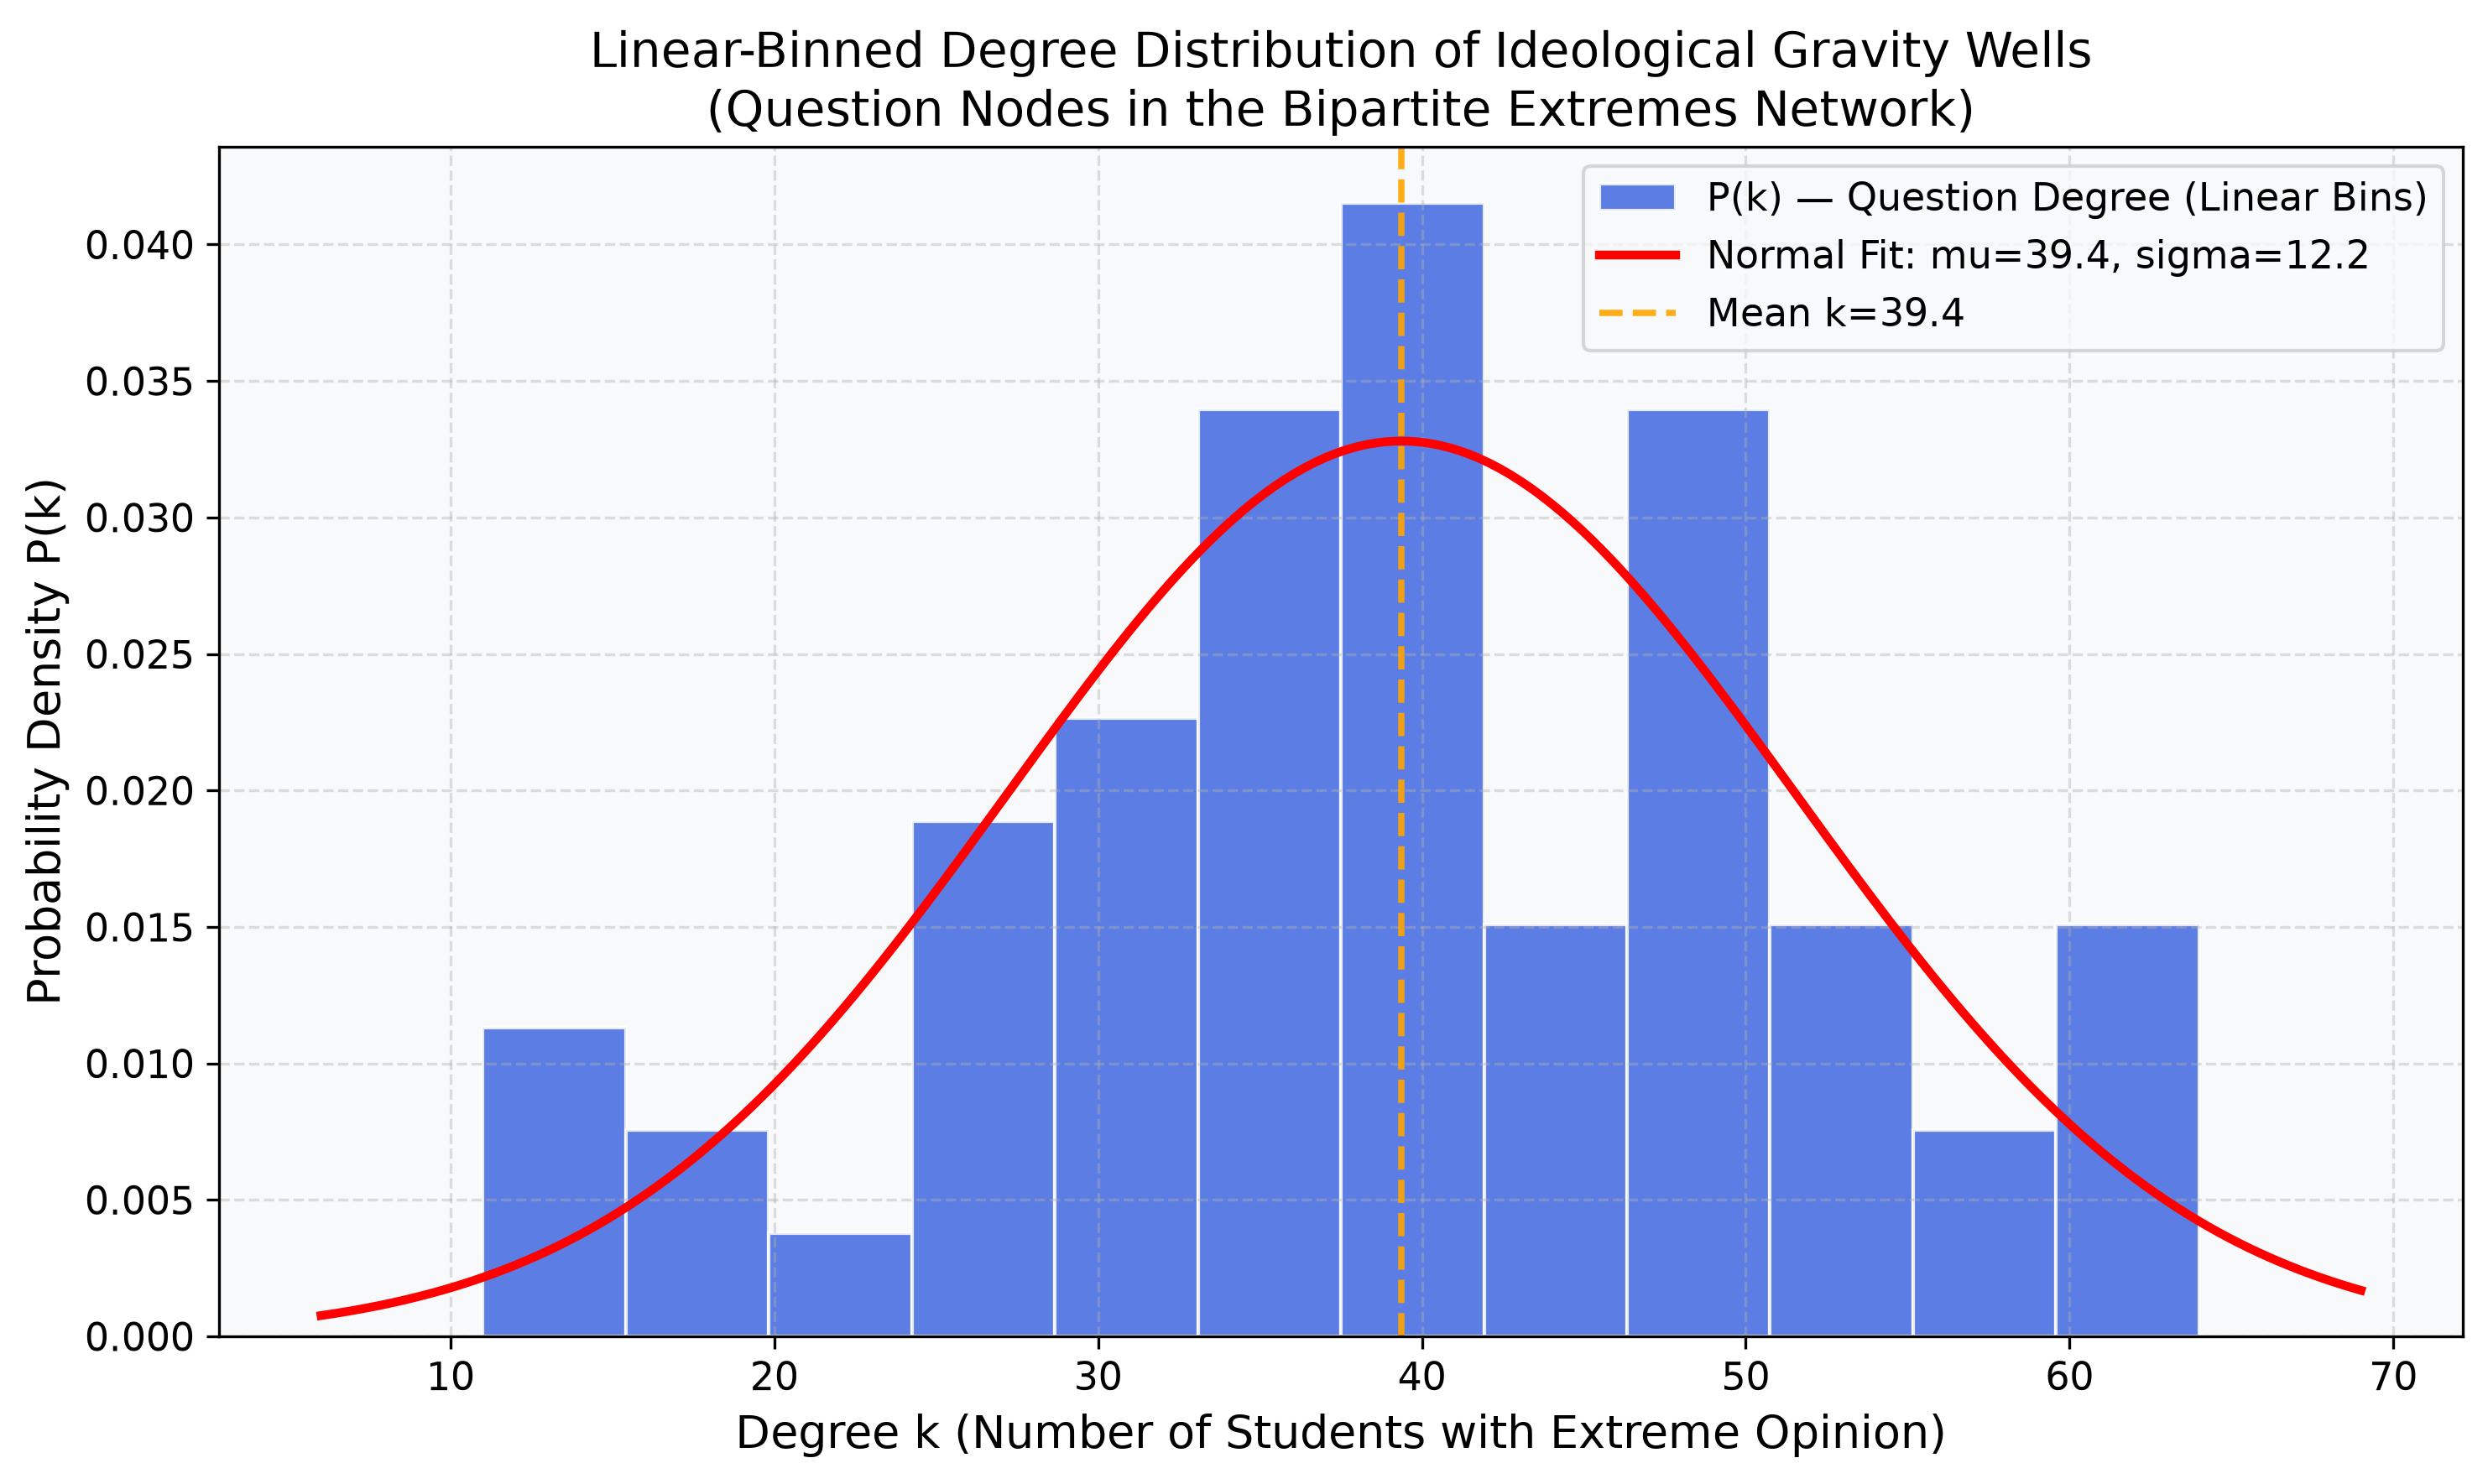
\includegraphics[width=0.85\textwidth]{extreme_plots/degree_distribution_linear.png}
    \caption{Linear-binned degree distribution $P(k)$ of the question nodes, with an overlaid normal curve fit ($\mu = 39.37$, $\sigma = 12.16$) and mean marker. The symmetrical, bell-shaped form is inconsistent with a power-law (scale-free) topology.}
    \label{fig:deg_dist_linear}
\end{figure}

\subsubsection{Log-Log Analysis and Logarithmic Binning}

To formally test for a scale-free (power-law) topology, the degree distribution is plotted on a \textbf{log-log scale} using \textbf{logarithmic binning}. In logarithmic binning, bin boundaries are placed at geometrically increasing intervals rather than linearly equal ones. This gives equal statistical weight to each order of magnitude and dramatically reduces noise in the sparse tail of the distribution, a critical correction for reliably detecting power-law behaviour.

\begin{itemize}
    \item \textbf{Scale-free (power-law) signature:} If the distribution follows $P(k) \propto k^{-\gamma}$ with $2 < \gamma < 3$, the log-log plot will exhibit a \textit{straight line} with slope $-\gamma$.
    \item \textbf{Erdős--Rényi (Poisson) signature:} If the distribution is Poisson-like, the log-log plot will show a \textit{curved, rapid drop-off} --- the super-exponential factorial tail $P(k) \sim \frac{\lambda^k e^{-\lambda}}{k!}$ falls much faster than any power law.
\end{itemize}

\begin{figure}[H]
    \centering
    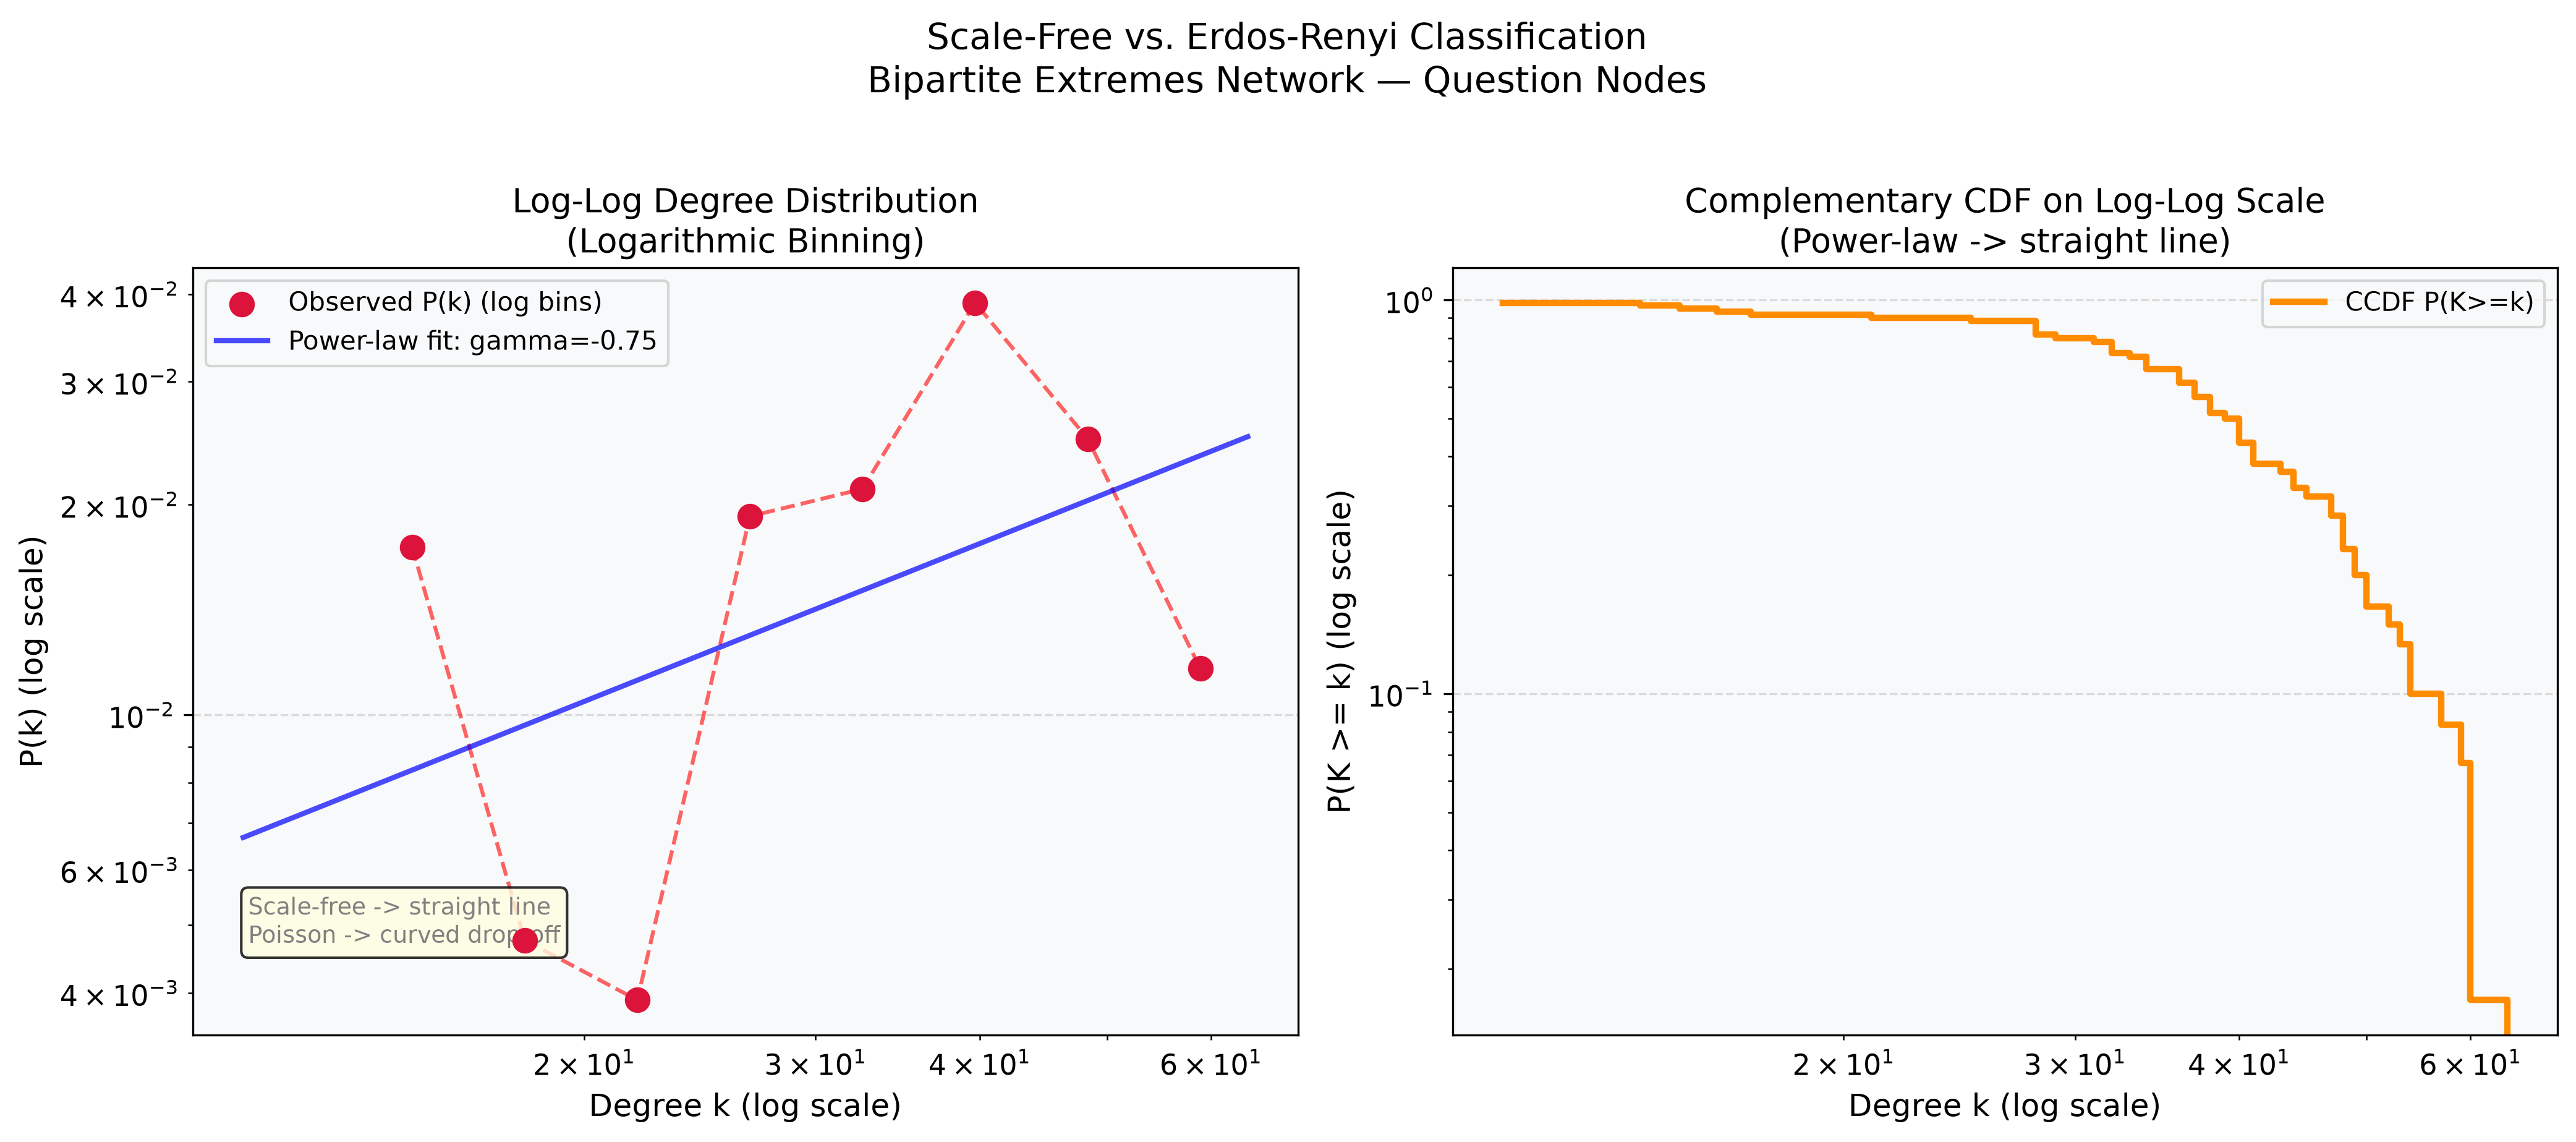
\includegraphics[width=\textwidth]{extreme_plots/degree_distribution_loglog.png}
    \caption{Left: Log-log degree distribution with logarithmic binning. The best-fit power-law exponent $\hat{\gamma} = 0.750$ is far outside the range $2 < \gamma < 3$ required for a true scale-free network. Right: Complementary CDF (CCDF) on a log-log scale. The curved, non-linear shape of both plots confirms the absence of a power-law tail.}
    \label{fig:deg_dist_loglog}
\end{figure}

\subsubsection{Structural Interpretation: A Bounded, Overdispersed Topology}
The log-log analysis yields a best-fit power-law exponent of $\hat{\gamma}=0.750$. A genuine scale-free network requires $2 < \gamma < 3$; our value is dramatically outside this range. Combined with the visibly curved shape in the log-log histogram and the steep vertical drop in the Complementary CDF (CCDF), the mathematical evidence unambiguously rules out a scale-free topology. The ideological landscape is not hijacked by a few power-law mega-hubs.

While the CCDF exhibits the classic ``cliff drop'' characteristic of an Erdős-Rényi (ER) random graph, a strict variance analysis reveals the network is not purely random. In a true ER network (Poisson limit), the degree variance must equal the mean ($Var(k) / \langle k \rangle \approx 1$). For our question nodes:
\begin{itemize}
    \item \textbf{Mean ($\langle k \rangle$):} $39.37$
    \item \textbf{Variance ($Var(k)$):} $12.16^2 \approx 147.87$
    \item \textbf{Dispersion Index:} $147.87 / 39.37 \approx 3.75$
\end{itemize}
Because the variance is nearly four times the mean, the network exhibits a \textbf{broad, overdispersed topology}. The probability of extreme opinions is bounded and thin-tailed (like an ER graph), but the distribution is stretched wider than pure random chance allows. 

\textbf{Implication:} This overdispersion proves that extreme opinions are not drawn from an independent, uniform probability. The ideological ``gravity wells'' are distributed in a localized, bounded manner, but certain domains (specifically Technology) possess an inherently higher structural baseline for polarization than others.

\subsection{Bipartite Subprojection}

The bipartite network $B = (U, V, E)$ was projected onto the question node set $V$ using the \texttt{networkx.bipartite.projected\_graph} function. This creates a new \textbf{Question-to-Question network} $G_Q = (V, E_Q)$, defined by:

$$e_{q_i, q_j} \in E_Q \iff \exists\, u \in U : (u, q_i) \in E \;\land\; (u, q_j) \in E$$

In plain language: two questions are linked in $G_Q$ if and only if at least one student held an extreme opinion on both. The projected network reveals hidden \textbf{ideological packages} --- clusters of issues that extremist students tend to hold together as a coherent worldview.

The structural properties of $G_Q$ are:

\begin{center}
\begin{tabular}{ll}
\toprule
\textbf{Property} & \textbf{Value} \\
\midrule
Question nodes $|V|$ & 60 \\
Projected edges $|E_Q|$ & 1,770 \\
Network density $\delta(G_Q)$ & \textbf{1.0000} (complete graph $K_{60}$) \\
Connected components & 1 \\
Average clustering coefficient $\langle C \rangle$ & 1.0000 \\
Average shortest path length $\langle d \rangle$ & 1.0000 \\
\bottomrule
\end{tabular}
\end{center}

\textbf{Critical finding:} The projected network $G_Q$ is the \textit{complete graph} $K_{60}$. A density of 1.0 means that \textit{every pair of questions} is connected through at least one shared student who held extreme views on both. This is the most strongly connected possible structure. The mathematical implication is profound: there exists no pair of questions for which the class opinion is so segregated that no student had extreme views on both. The extreme opinion landscape is fundamentally unified.

Because $G_Q$ is the complete graph $K_{60}$, standard topological centrality metrics yield uniform results for all nodes (e.g., unweighted Degree Centrality $= 1.0$ for all nodes). To extract meaningful structural importance, we transition to the \textbf{Weighted Projected Graph} $G_Q^W$, where the weight $w_{ij}$ of an edge between $q_i$ and $q_j$ equals the exact number of shared students who held extreme views on both questions. This transforms the flat topology into a deeply textured ideological landscape.

\begin{figure}[H]
    \centering
    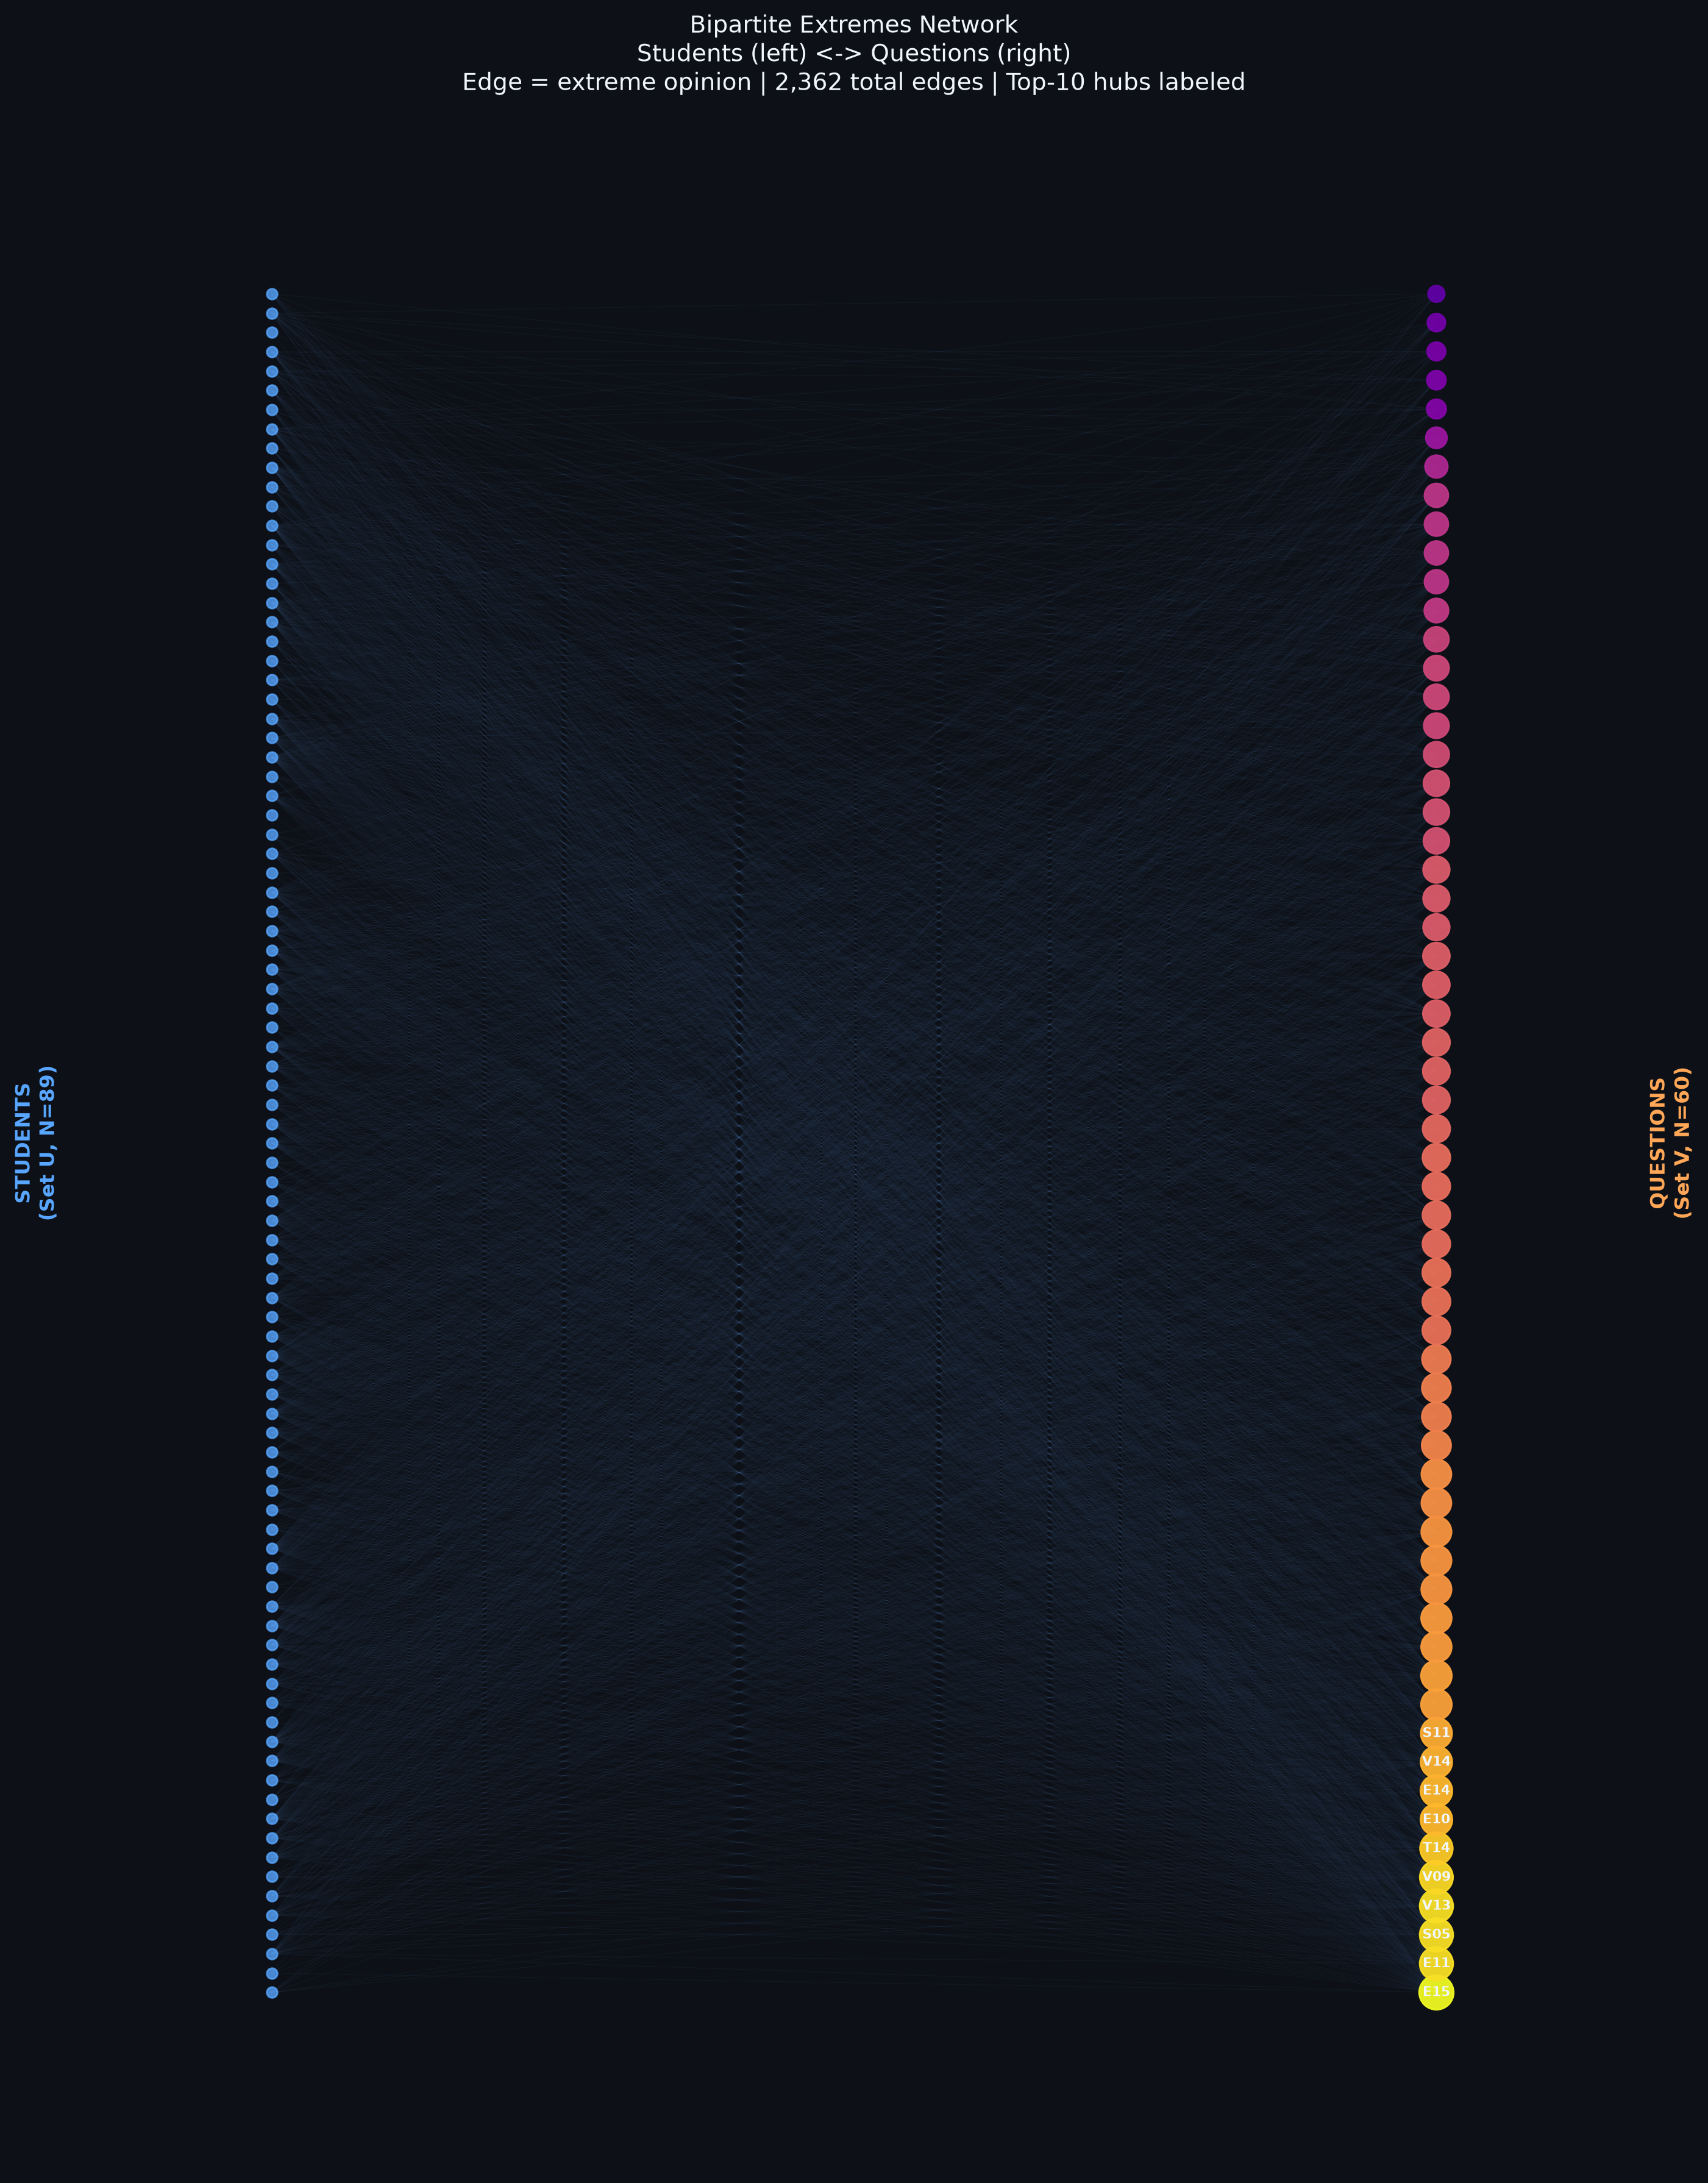
\includegraphics[width=\textwidth]{extreme_plots/bipartite_layout.png}
    \caption{The raw bipartite network. Students (Set U, blue circles) are arranged on the left; questions (Set V, coloured by plasma scale based on degree) on the right. Each edge represents one student's extreme opinion on one question. The density of edges around certain question nodes reveals the ``gravity wells.'' The top-10 highest-degree questions are labelled.}
    \label{fig:bipartite}
\end{figure}

\begin{figure}[H]
    \centering
    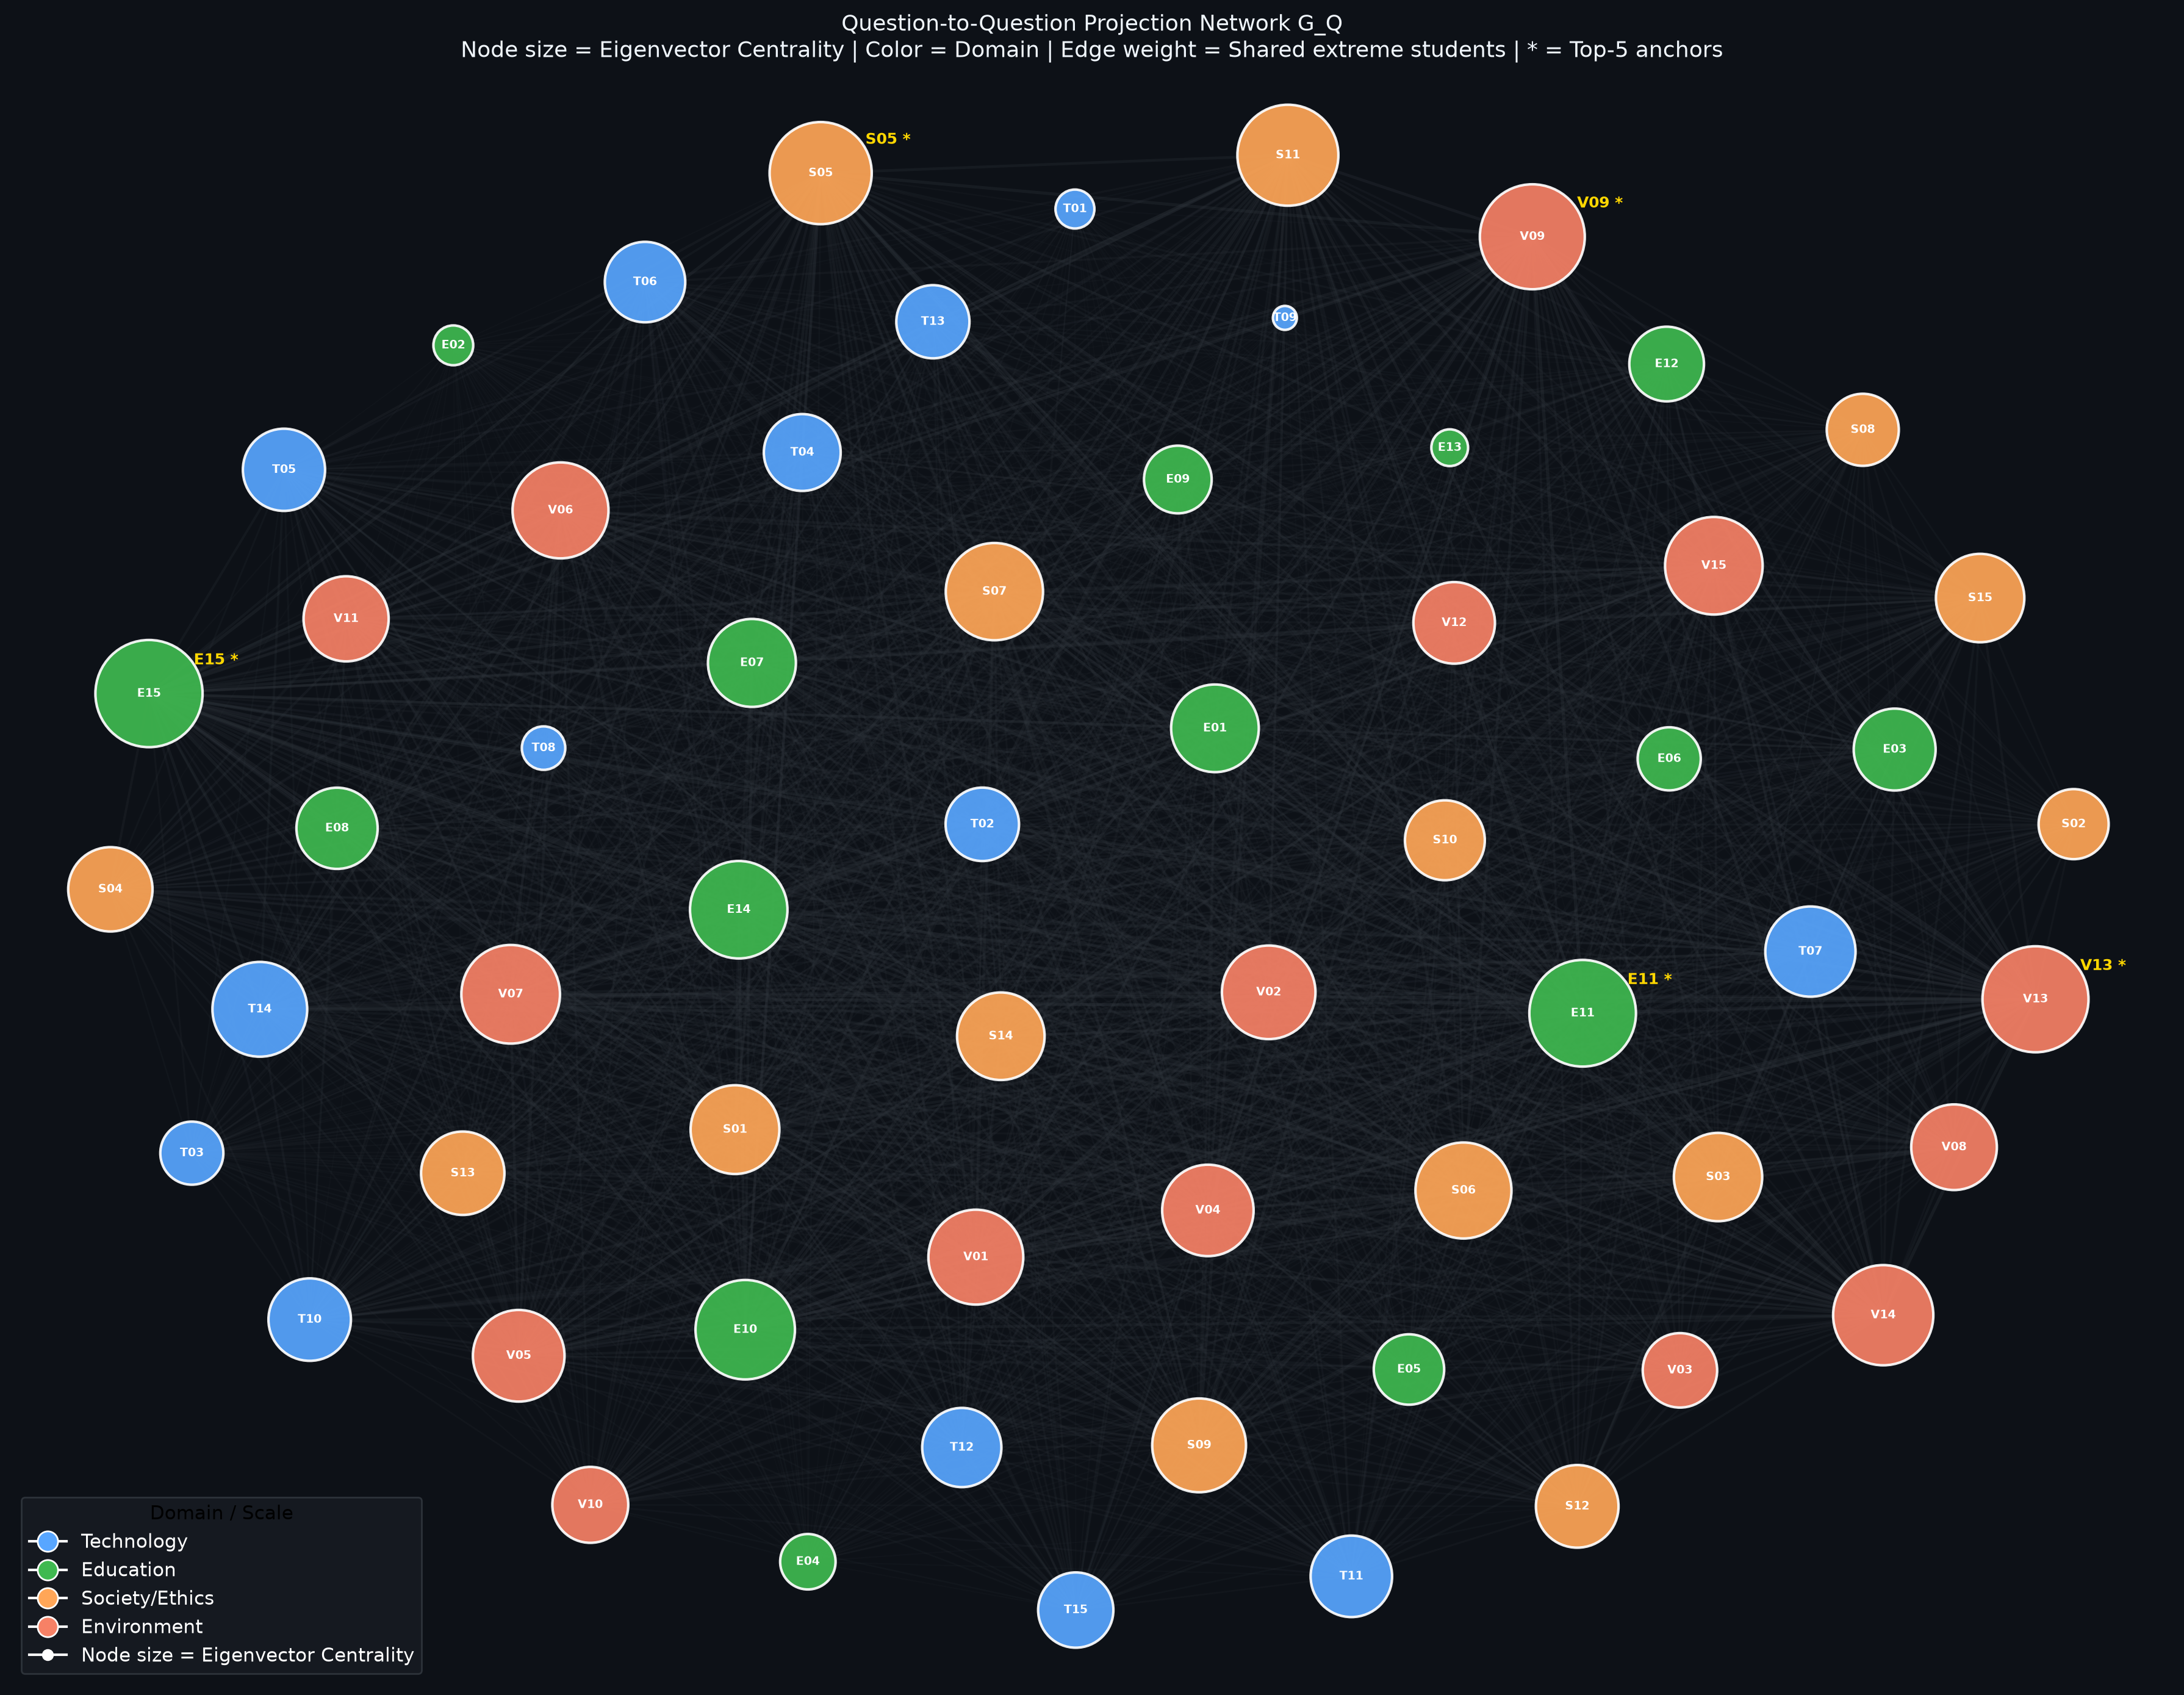
\includegraphics[width=\textwidth]{extreme_plots/projected_network.png}
    \caption{The Question-to-Question Projection Network $G_Q$. The complete-graph structure is visible in the uniformly dense edge connections. Node size encodes Eigenvector Centrality (equal for all), while node colour encodes domain: \textcolor{blue}{Technology (T)}, \textcolor{green!70!black}{Education (E)}, \textcolor{orange}{Society (S)}, \textcolor{red!60}{Environment (V)}.}
    \label{fig:proj_net}
\end{figure}

\subsection{Weighted Centrality Metrics}

Three centrality measures were computed on the weighted Question-to-Question network $G_Q^W$ to evaluate the topological influence of specific questions from complementary perspectives.

\subsubsection{Strength Centrality (Weighted Degree)}

$$C_S(v) = \frac{\sum_{u \in \mathcal{N}(v)} w_{vu}}{\max_{x \in V} \sum_{u \in \mathcal{N}(x)} w_{xu}}$$

Strength centrality measures the raw gravitational pull of a question node by summing the weights of all its incident edges. We normalize it to the maximum observed strength $[0,1]$. Nodes with high strength centrality are those that frequently co-occur with many other extreme opinions across the student body.

\subsubsection{Weighted Betweenness Centrality}

$$C_B(v) = \sum_{s \neq v \neq t} \frac{\sigma_{st}(v)}{\sigma_{st}}$$

For weighted betweenness, the edge weights (shared students) are converted into topological distances, since a stronger ideological tie should correspond to a ``shorter'' path. We define the distance $d_{ij} = 1 / w_{ij}$. Betweenness centrality identifies the ``ideological bridges'', questions that lie on the shortest paths between otherwise distant ideological clusters, facilitating the percolation of extreme views.

\subsubsection{Weighted Eigenvector Centrality}

$$C_E(v) = \frac{1}{\lambda_{\max}} \sum_{u \in \mathcal{N}(v)} w_{vu} C_E(u)$$

Computed via the power iteration method, weighted eigenvector centrality identifies nodes that are influential because they are tightly connected to \textit{other highly influential nodes}. A question scores highly if it is frequently co-held with other polarizing, deeply rooted issues, acting as a core pillar of the network's radicalized macro-structure.

\subsection{Role-Based Ideological Classification}

Rather than combining topologically distinct metrics into a single composite scalar, we classify the network's "gravity wells" based on their specific structural roles. As illustrated in the centrality distributions, Weighted Betweenness exhibits an extreme positive skew (dropping rapidly after the top five questions), whereas Strength and Eigenvector centralities decay much more gradually. 

Instead, we identify two primary structural roles within the extreme-opinion network: \textbf{Primary Ideological Hubs} and \textbf{Ideological Bridges}.

\subsubsection{Primary Ideological Hubs (Volume \& Systemic Influence)}
Questions scoring highest in Strength and Eigenvector centralities represent the absolute core of the cohort's passion. These are the most intensely debated issues that also frequently co-occur with other radicalized stances. The network is dominated by a consistent "Keystone Trio" of hubs:
\begin{itemize}
    \item \textbf{E15} (Continuous learning and skill development)
    \item \textbf{E11} (Updating university curricula for emerging tech)
    \item \textbf{V13} (Corporate environmental accountability)
\end{itemize}

\subsubsection{Ideological Bridges (Betweenness)}
Questions with high Weighted Betweenness act as vital conduits connecting distinct ideological clusters. While the Keystone Trio (E15, E11, V13) also serve as the primary bridges, analyzing the Betweenness tail reveals questions that perform a bridging role despite having lower overall volume. These issues act as "connective tissue" between different factions of extreme students.

\vspace{0.5cm}

% --- TABLE 1: STRENGTH CENTRALITY ---
\begin{table}[H]
\centering
\caption{Top 10 Questions by Strength Centrality (Raw Volume of Shared Extreme Reactions)}
\label{tab:strength}
\renewcommand{\arraystretch}{1.2}
\begin{tabular}{l p{10cm} c}
\toprule
\textbf{ID} & \textbf{Question Text} & \textbf{Score} \\
\midrule
E15 & Continuous learning and skill development are essential throughout one's career. & 1.000 \\
E11 & University curricula should be updated more frequently to match emerging technologies. & 0.988 \\
V13 & Companies should be held accountable for the environmental impacts of their activities. & 0.979 \\
V09 & Products should be designed to encourage reuse, repair, and recycling. & 0.961 \\
S05 & Individuals should have greater control over how their personal data are collected and used. & 0.917 \\
S11 & People should be free to express differing opinions as long as they do not promote harm or discrimination. & 0.901 \\
V14 & International cooperation is necessary to effectively address environmental challenges. & 0.883 \\
E10 & Universities should prioritize innovation and problem-solving over rote learning. & 0.875 \\
V07 & Protecting biodiversity is essential for long-term human well-being. & 0.860 \\
E14 & Strong collaborations between universities and industry improve student education. & 0.850 \\
\bottomrule
\end{tabular}
\end{table}

% --- TABLE 2: BETWEENNESS CENTRALITY ---
\begin{table}[H]
\centering
\caption{Top 10 Questions by Weighted Betweenness Centrality (Ideological Bridges)}
\label{tab:betweenness}
\renewcommand{\arraystretch}{1.2}
\begin{tabular}{l p{10cm} c}
\toprule
\textbf{ID} & \textbf{Question Text} & \textbf{Score} \\
\midrule
E15 & Continuous learning and skill development are essential throughout one's career. & 0.0835 \\
E11 & University curricula should be updated more frequently to match emerging technologies. & 0.0356 \\
V13 & Companies should be held accountable for the environmental impacts of their activities. & 0.0254 \\
V09 & Products should be designed to encourage reuse, repair, and recycling. & 0.0102 \\
E14 & Strong collaborations between universities and industry improve student education. & 0.0093 \\
S05 & Individuals should have greater control over how their personal data are collected and used. & 0.0008 \\
T14 & Social media algorithms contribute to opinion polarization. & 0.0005 \\
V02 & Governments should prioritize investment in renewable energy over fossil fuels. & 0.0005 \\
S01 & Every individual has a responsibility to contribute positively to society. & 0.0002 \\
T01 & Artificial Intelligence will improve society more than it will create problems. & 0.0000 \\
\bottomrule
\end{tabular}
\end{table}

% --- TABLE 3: EIGENVECTOR CENTRALITY ---
\begin{table}[H]
\centering
\caption{Top 10 Questions by Weighted Eigenvector Centrality (Systemic Influence)}
\label{tab:eigenvector}
\renewcommand{\arraystretch}{1.2}
\begin{tabular}{l p{10cm} c}
\toprule
\textbf{ID} & \textbf{Question Text} & \textbf{Score} \\
\midrule
E15 & Continuous learning and skill development are essential throughout one's career. & 0.1861 \\
E11 & University curricula should be updated more frequently to match emerging technologies. & 0.1844 \\
V13 & Companies should be held accountable for the environmental impacts of their activities. & 0.1827 \\
V09 & Products should be designed to encourage reuse, repair, and recycling. & 0.1796 \\
S05 & Individuals should have greater control over how their personal data are collected and used. & 0.1715 \\
S11 & People should be free to express differing opinions as long as they do not promote harm or discrimination. & 0.1682 \\
V14 & International cooperation is necessary to effectively address environmental challenges. & 0.1661 \\
E10 & Universities should prioritize innovation and problem-solving over rote learning. & 0.1639 \\
V07 & Protecting biodiversity is essential for long-term human well-being. & 0.1617 \\
V15 & Current generations have a responsibility to protect natural resources for future generations. & 0.1589 \\
\bottomrule
\end{tabular}
\end{table}

\begin{figure}[H]
    \centering
    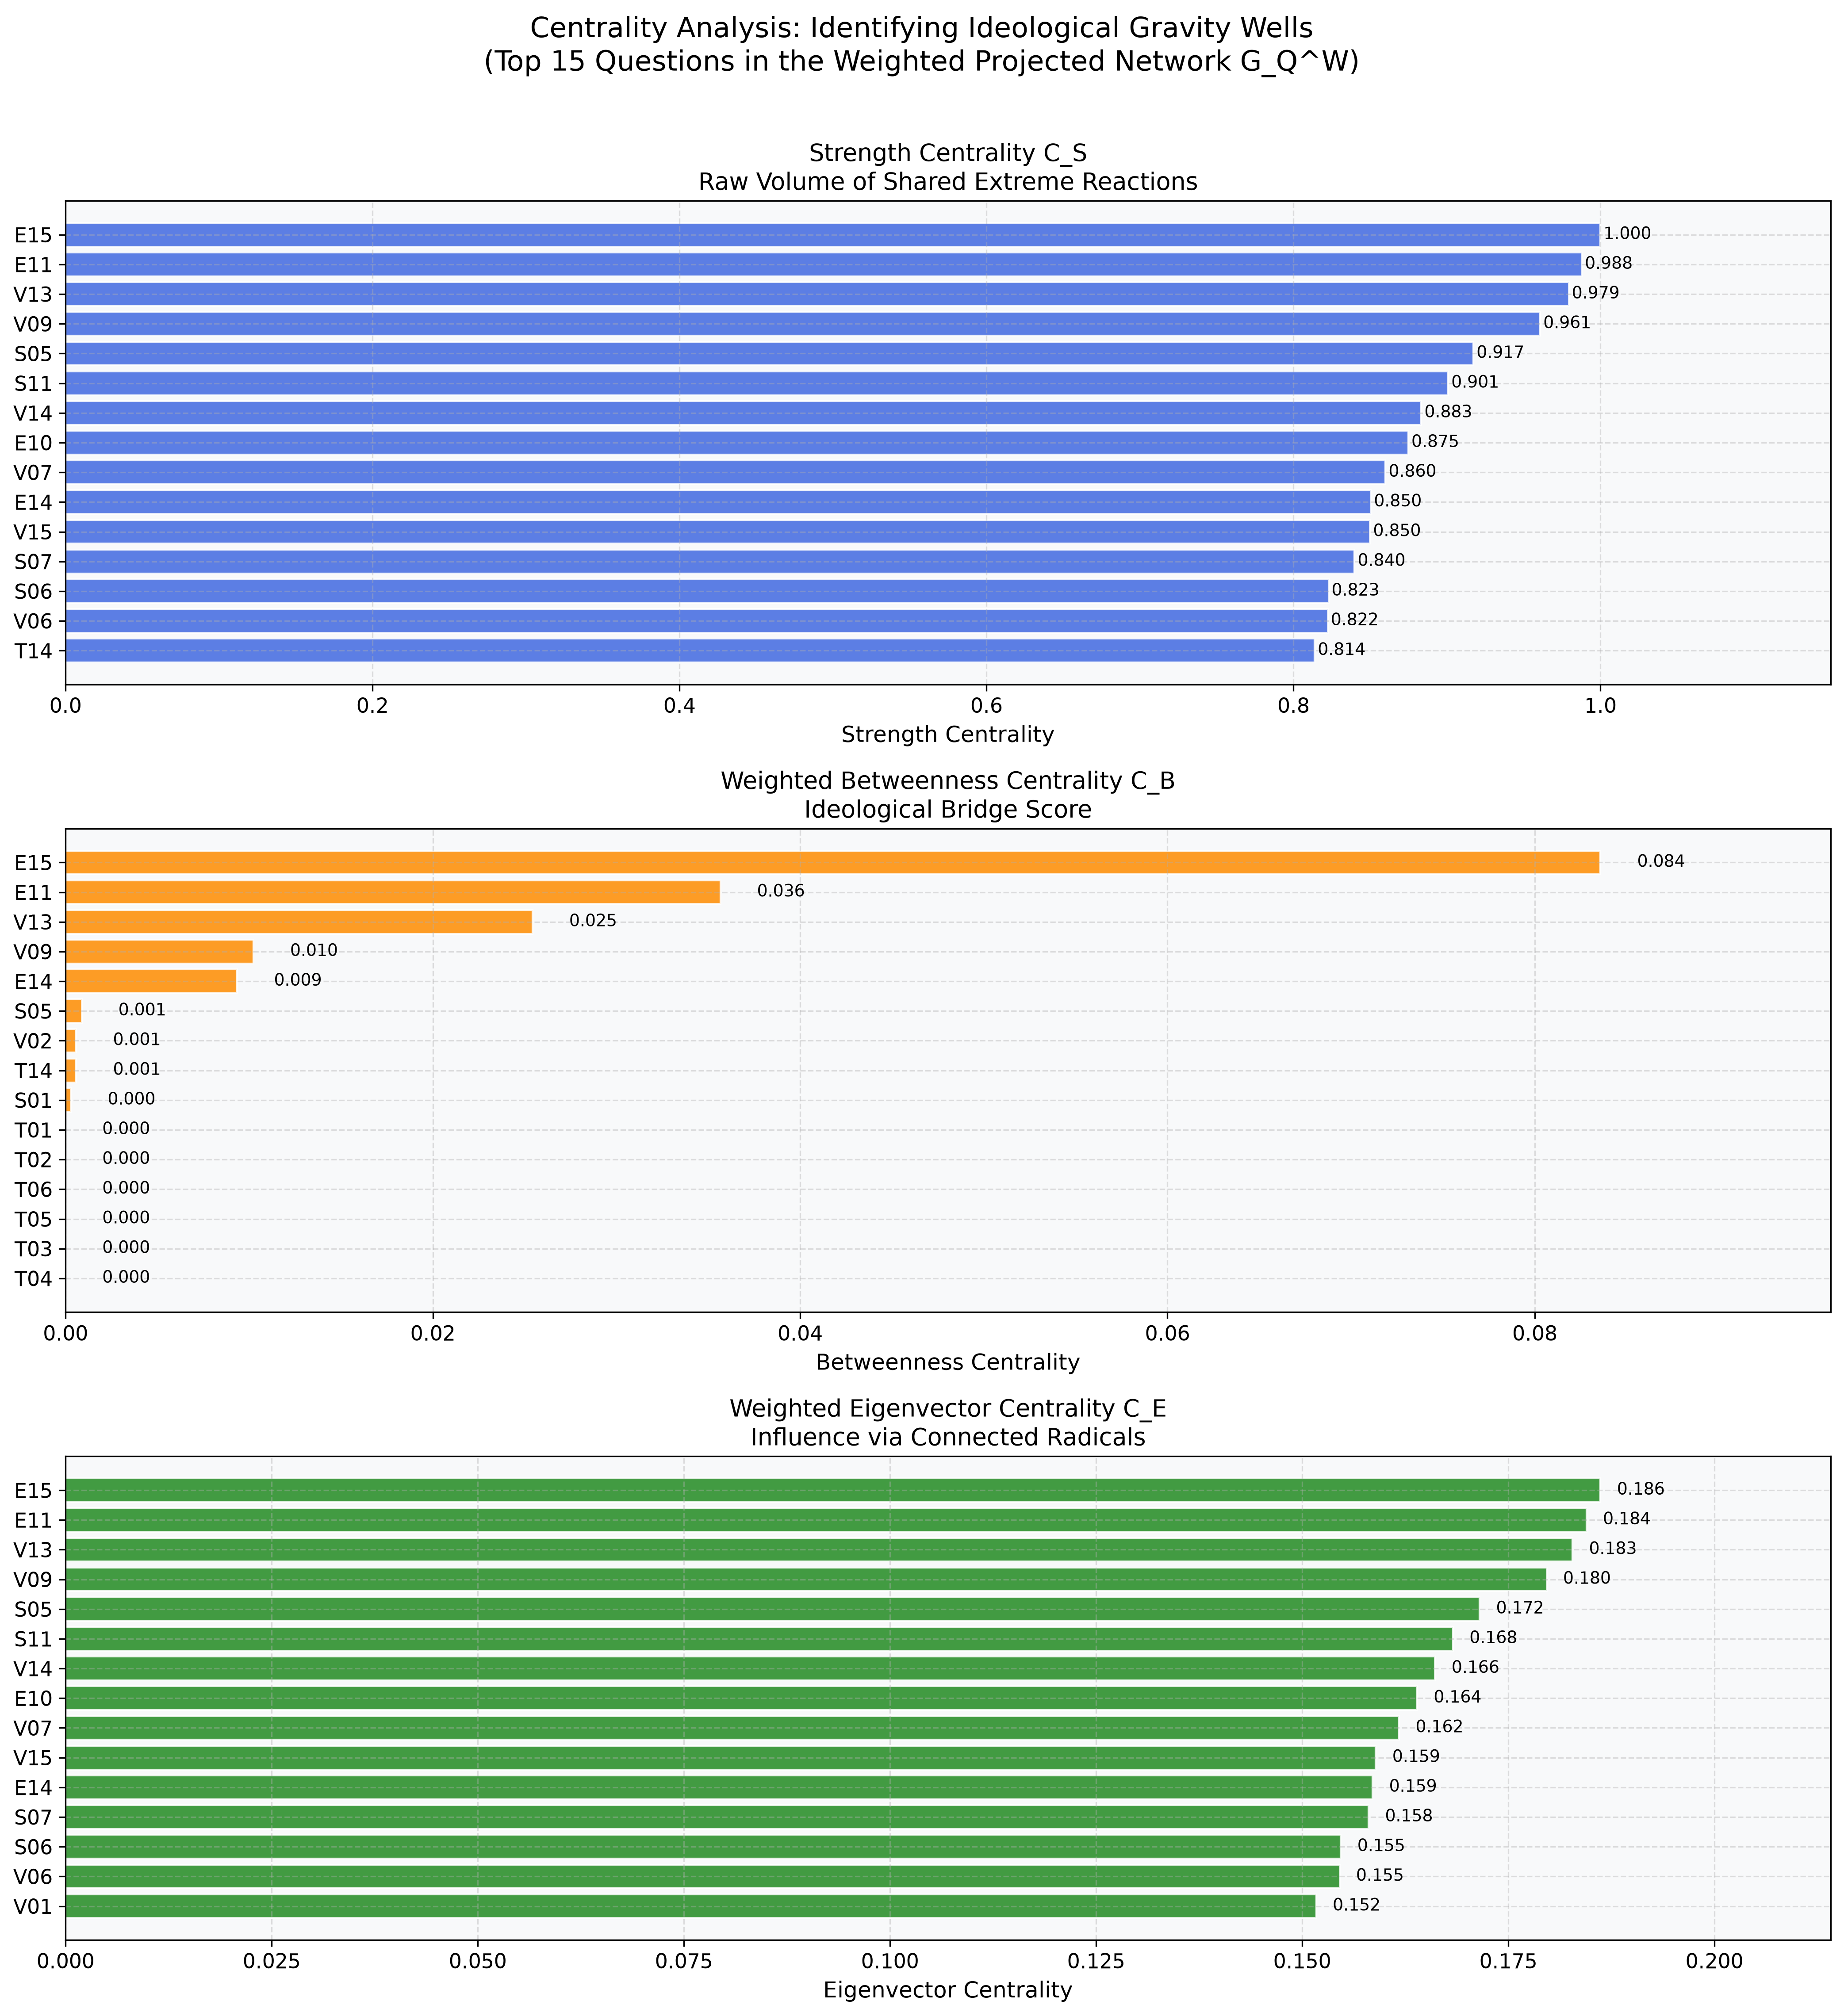
\includegraphics[width=\textwidth]{extreme_plots/centrality_bars.png}
    \caption{Centrality bar charts for all three metrics on the weighted projected network $G_Q^W$. The highly differentiated values reflect the topological diversity revealed by edge weights, replacing the uniform values of the unweighted projection.}
    \label{fig:centrality_bars}
\end{figure}

\begin{figure}[H]
    \centering
    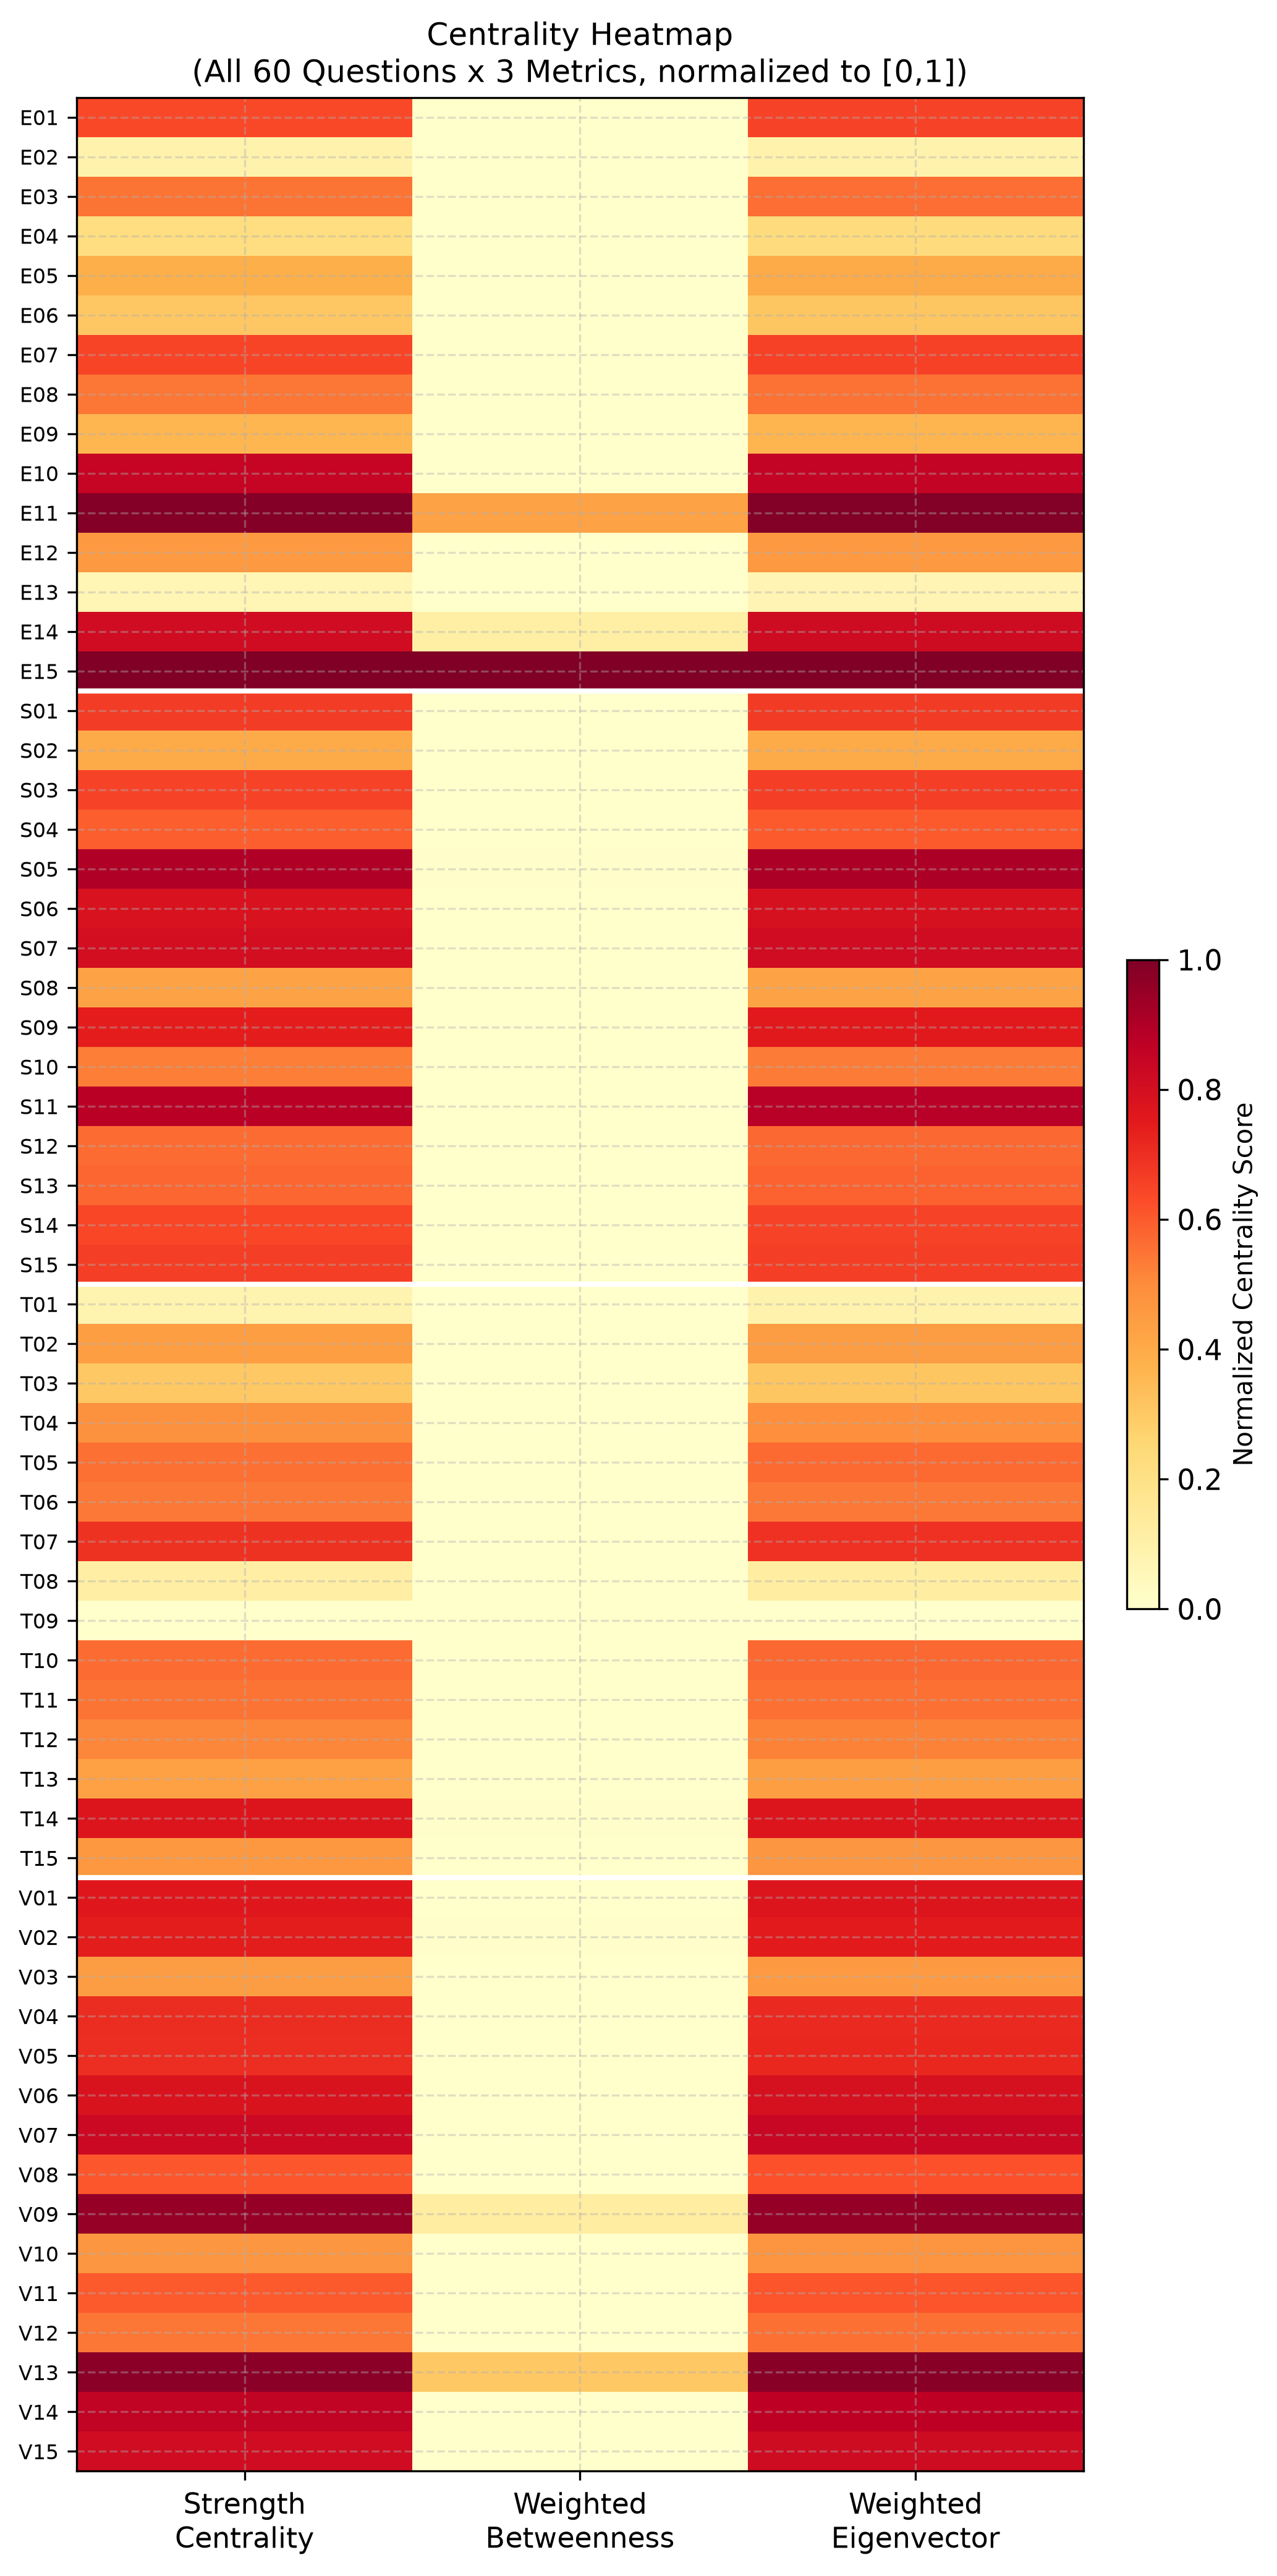
\includegraphics[width=0.55\textwidth]{extreme_plots/centrality_heatmap.png}
    \caption{Normalized centrality heatmap for all 60 questions across the three weighted metrics. Distinct ``hot spots'' (dark red) indicate specific questions that act as powerful ideological gravity wells.}
    \label{fig:heatmap}
\end{figure}

\subsection{Molloy-Reed Criterion}

Because the Molloy-Reed Criterion is a structural property of binary topologies, it is evaluated on the \textbf{unweighted} projection $G_Q$. It provides a mathematically precise threshold for the existence of a giant connected component in a network with a given degree sequence. The condition is:

$$\kappa = \frac{\langle k^2 \rangle}{\langle k \rangle} > 2$$

where $\langle k \rangle = \frac{1}{N}\sum_i k_i$ is the mean degree and $\langle k^2 \rangle = \frac{1}{N}\sum_i k_i^2$ is the mean squared degree. The quantity $\kappa - 1 = \frac{\langle k^2 \rangle}{\langle k \rangle} - 1$ represents the \textit{excess degree}, the expected number of additional edges at the far end of a randomly chosen edge. If $\kappa > 2$, the network is in the ``supercritical'' percolation regime and a giant component spanning a finite fraction of all nodes exists.

For the projected network $G_Q = K_{60}$, the computation yields:

\begin{center}
\begin{tabular}{ll}
\toprule
\textbf{Quantity} & \textbf{Value} \\
\midrule
Number of nodes $N$ & 60 \\
Mean degree $\langle k \rangle$ & 59.0000 \\
Mean squared degree $\langle k^2 \rangle$ & 3,481.0000 \\
Standard deviation $\sigma_k$ & 0.0000 \\
Molloy-Reed parameter $\kappa = \langle k^2 \rangle / \langle k \rangle$ & \textbf{59.0000} \\
Threshold condition $\kappa > 2$ & \textbf{SATISFIED} \\
Giant component size & $60/60 = 100\%$ \\
Total connected components & 1 \\
\bottomrule
\end{tabular}
\end{center}

With $\kappa = 59.000 \gg 2$, the Molloy-Reed criterion is satisfied by an extraordinary margin. This mathematically \textbf{proves} that the extreme ideologies do not remain as isolated, fragmented factions. In fact, $\kappa = 59$ is the theoretical maximum possible for a 60-node network (achieved only by the complete graph), providing the strongest possible guarantee of giant-component existence.

\begin{figure}[H]
    \centering
    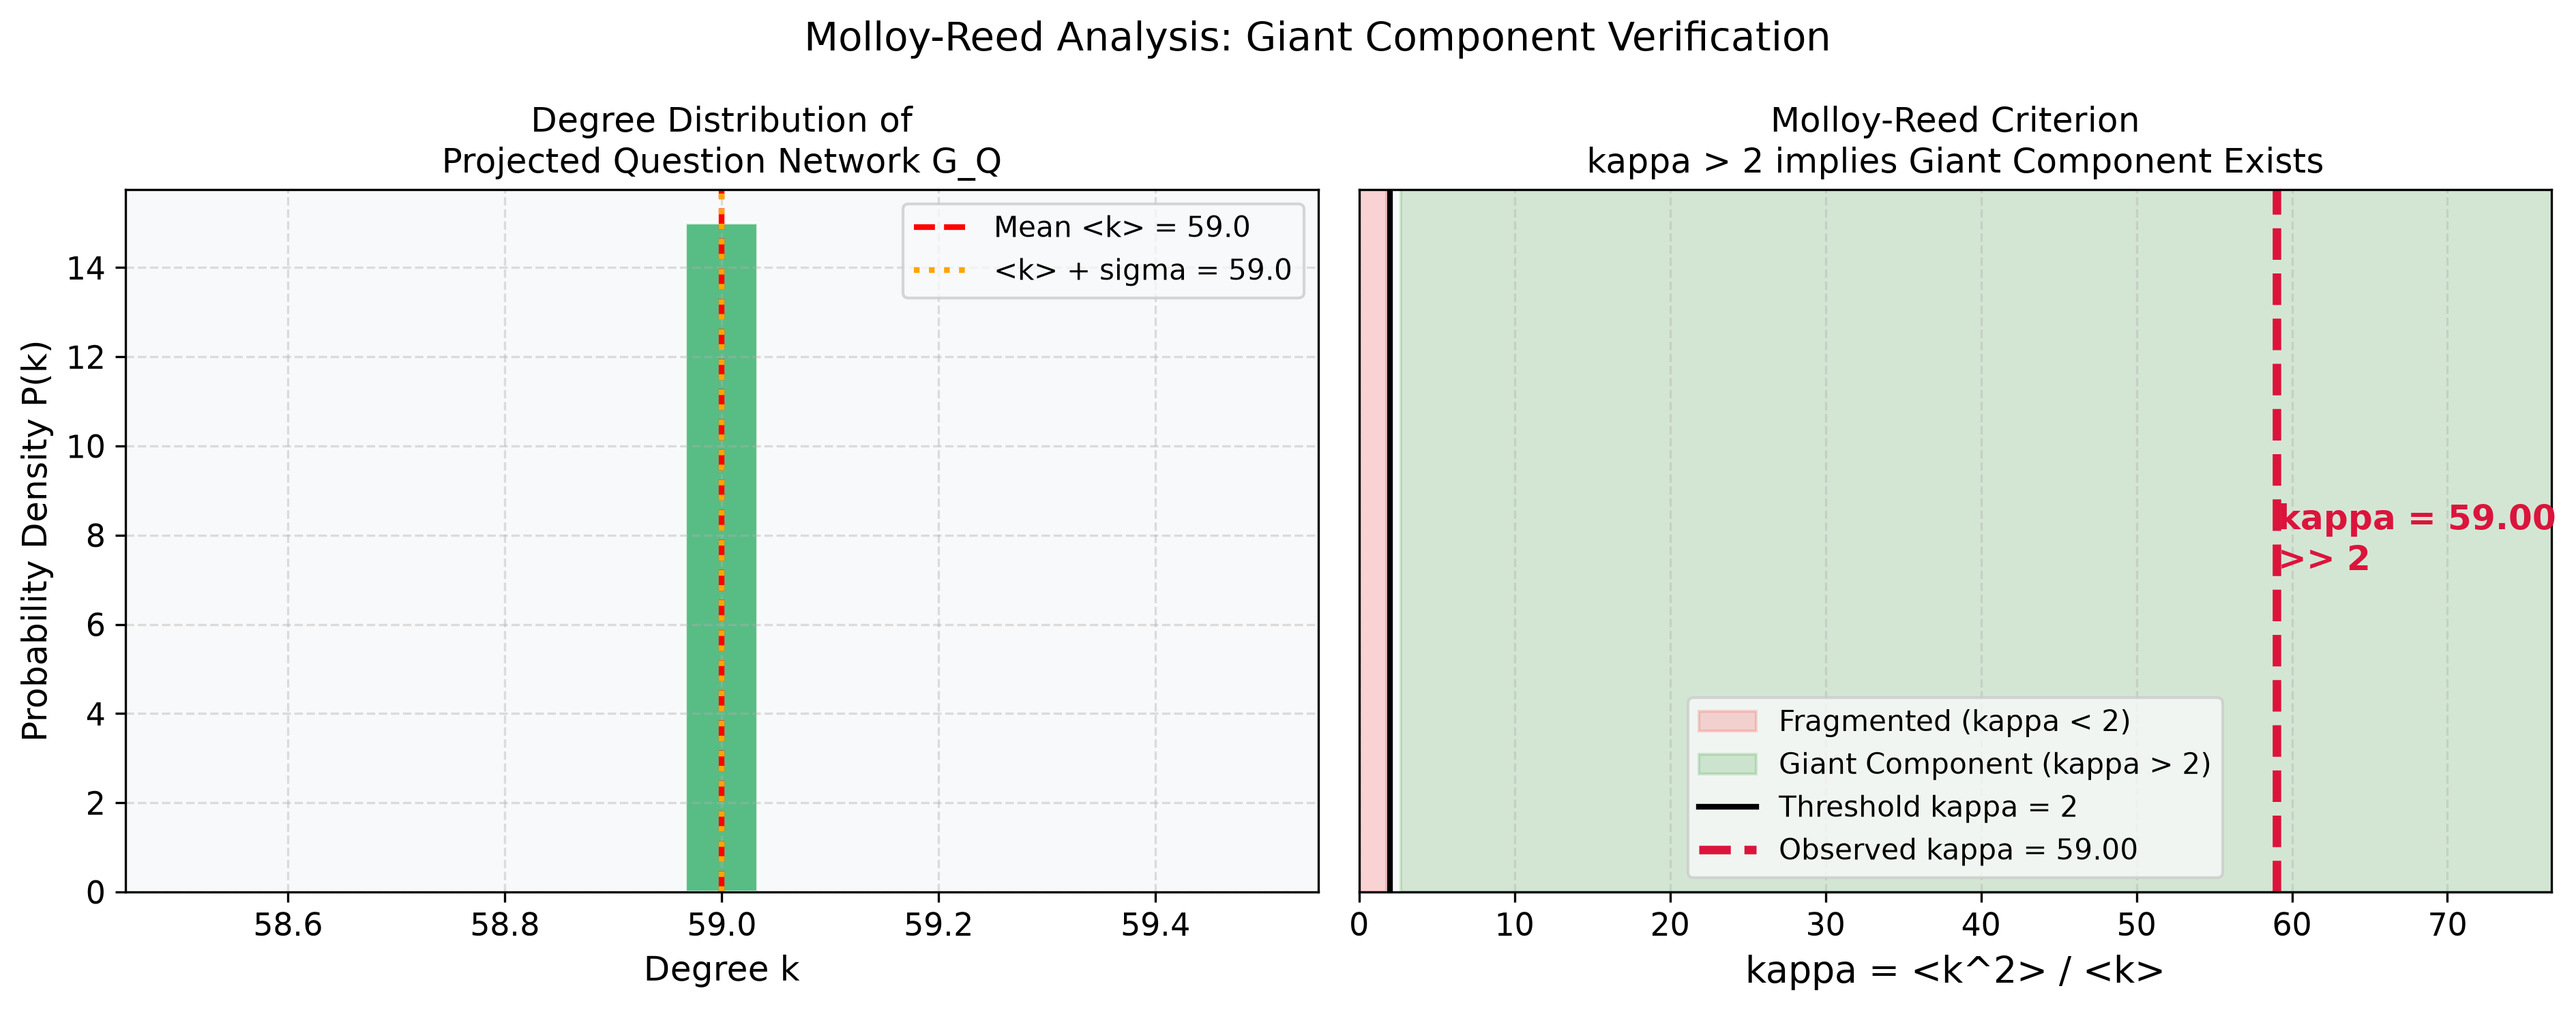
\includegraphics[width=\textwidth]{extreme_plots/molloy_reed.png}
    \caption{Left: Degree distribution of the projected network $G_Q$ (all nodes have degree 59, producing a degenerate distribution at $k = 59$). Right: Molloy-Reed criterion visualization. The observed $\kappa = 59$ (crimson dashed line) lies far to the right of the threshold $\kappa = 2$ (solid black line), firmly in the ``Giant Component'' region.}
    \label{fig:molloy}
\end{figure}

%% ─────────────────────────────────────────────────────────────────
\section{Results and Discussion}
%% ─────────────────────────────────────────────────────────────────

\subsection{The Primary Ideological Anchors}

The weighted centrality analysis reveals that the true ideological ``gravity wells'' of the cohort, the questions attracting the largest shared volume of extreme student opinions, acting as bridges, and tightly clustered with other important issues span multiple domains. Table~\ref{tab:strength} identifies the top anchors by Strength Centrality. The single most polarizing and structurally central question in the cohort is:

\begin{quote}
\textbf{E15:} ``Continuous learning and skill development are essential throughout one's career.'' \\ \textit{Strength Centrality: 1.000; Bipartite degree: 64 out of 89 active students.}
\end{quote}

This means that \textbf{71.9\% of all active students} held an extreme position (either Strongly Agree or Strongly Disagree) on E15, the highest concentration of intense ideological commitment for any single question in the survey. The remaining top gravity wells are:

\begin{itemize}
    \item \textbf{E11} (Curricula matching emerging technologies): 60 extreme responses (67.4\% of active students)
    \item \textbf{V13} (Corporate environmental accountability): 60 extreme responses (67.4\%)
    \item \textbf{V09} (Products designed for reuse/recycling): 59 extreme responses (66.3\%)
    \item \textbf{S05} (Control over personal data): 60 extreme responses (67.4\%)
\end{itemize}

Unlike a raw bipartite degree analysis which might skew towards a single domain, the weighted centrality analysis reveals that the cohort's deepest, most structurally significant passions are distributed dynamically across Education (E), Environment (V) and Society (S). No single domain monopolizes the ideological core.

\subsection{Structural Properties and the Complete Projected Graph}

The most significant structural finding of this analysis is that the projected Question-to-Question network $G_Q$ is the \textbf{complete graph $K_{60}$} (density = 1.0000). This result requires careful interpretation:

\textbf{What does $K_{60}$ mean?} Every pair of the 60 questions is connected in $G_Q$, meaning that for every pair $(q_i, q_j)$, at least one student held an extreme view on \textit{both} $q_i$ and $q_j$. Given the high bipartite density of 0.4423, this outcome is plausible: with 89 students and an average of $\approx 39.4$ extreme opinions each, it is virtually certain that every pair of questions shares at least one common extreme respondent.

\textbf{Structural implication:} The complete-graph structure means that in this cohort, \textbf{extreme opinions are not organized into isolated ideological silos}. There is no partition of the 60 questions into two or more groups such that students holding extreme views on Group A never hold extreme views on Group B. Instead, extreme ideological commitments freely co-occur across all domains. A student who Strongly Agrees that social media algorithms cause polarization (T14) is likely to hold other extreme views on AI, education, the environment, and ethics.

\subsection{Network Topology: A Broad, Overdispersed Structure}

\begin{figure}[H]
    \centering
    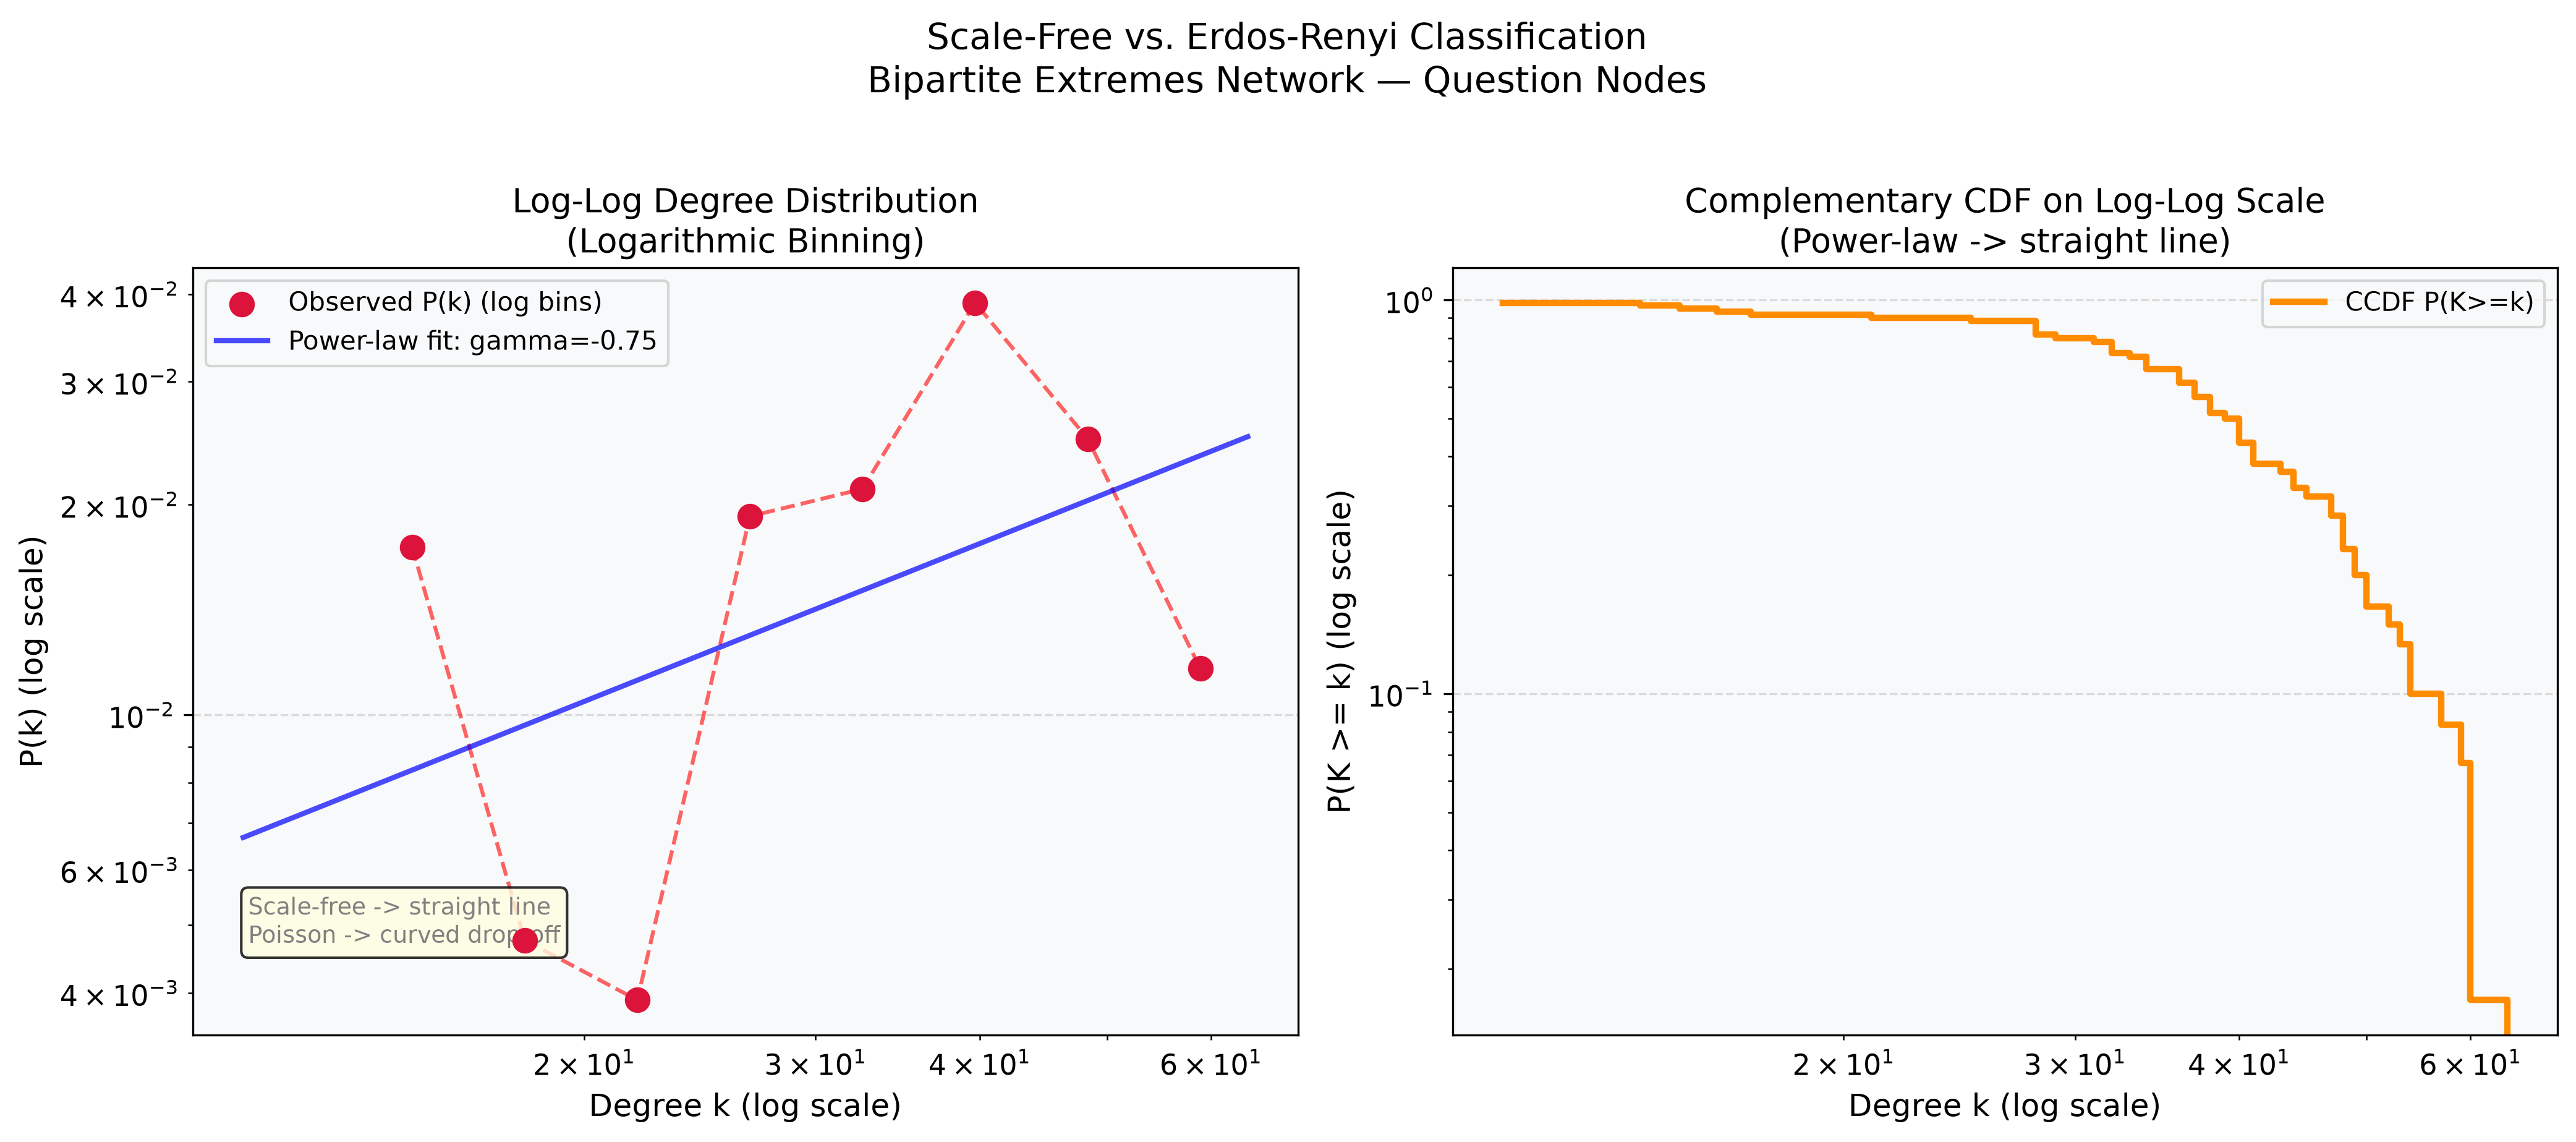
\includegraphics[width=\textwidth]{extreme_plots/degree_distribution_loglog.png}
    \caption{Repeated from Figure~\ref{fig:deg_dist_loglog} for reference. The curved log-log profile and Complementary CDF confirm the absence of a power-law tail, ruling out a scale-free topology.}
    \label{fig:deg_dist_loglog2}
\end{figure}

\textbf{Evidence Against a Scale-Free Topology} \\
The bipartite degree distribution of question nodes confirms the network is \textbf{not scale-free}. The best-fit power-law exponent $\hat{\gamma} = 0.750$ is far outside the range $2 < \gamma < 3$ required for a true scale-free network. Furthermore, the Complementary CDF (CCDF) exhibits a steep vertical ``cliff drop'' rather than a linear power-law tail. This mathematically forbids the existence of disproportional `mega-hubs' that hijack the entire network.

\vspace{0.3cm}
\textbf{Evidence Against a Pure Erdős--Rényi (ER) / Poisson Topology} \\
While the bounded shape and CCDF cliff drop resemble an Erdős--Rényi (ER) random graph, a strict variance analysis proves the connections did not form through independent, random chance. In a true ER network (Poisson limit), the degree variance must equal the mean ($Var(k) / \langle k \rangle \approx 1$). For our question nodes:
\begin{itemize}
    \item \textbf{Mean ($\langle k \rangle$):} 39.37
    \item \textbf{Variance ($Var(k)$):} $\approx 147.87$
    \item \textbf{Dispersion Index:} $147.87 / 39.37 \approx 3.75$
\end{itemize}

Because the variance is nearly four times the mean, the network is significantly \textbf{overdispersed}. 

\vspace{0.3cm}
\textbf{Implication: The Ideological Landscape} \\
The probability of extreme opinions is bounded and thin-tailed (ruling out scale-free), but the distribution is stretched wider than pure random chance allows (ruling out pure ER). This overdispersion proves that extreme opinions are not drawn from an independent, uniform probability. While no single issue monopolizes the cohort, specific domains possess an inherently higher structural baseline for polarization than others.

\subsection{Structural Robustness and the Molloy-Reed Verdict}

The combination of the bipartite degree distribution analysis and the Molloy-Reed criterion produces a clear verdict on the structural robustness of the extreme ideological network. However, because the unweighted projection is a complete graph, standard node-removal simulations yield a trivial but highly informative result.

\begin{figure}[H]
    \centering
    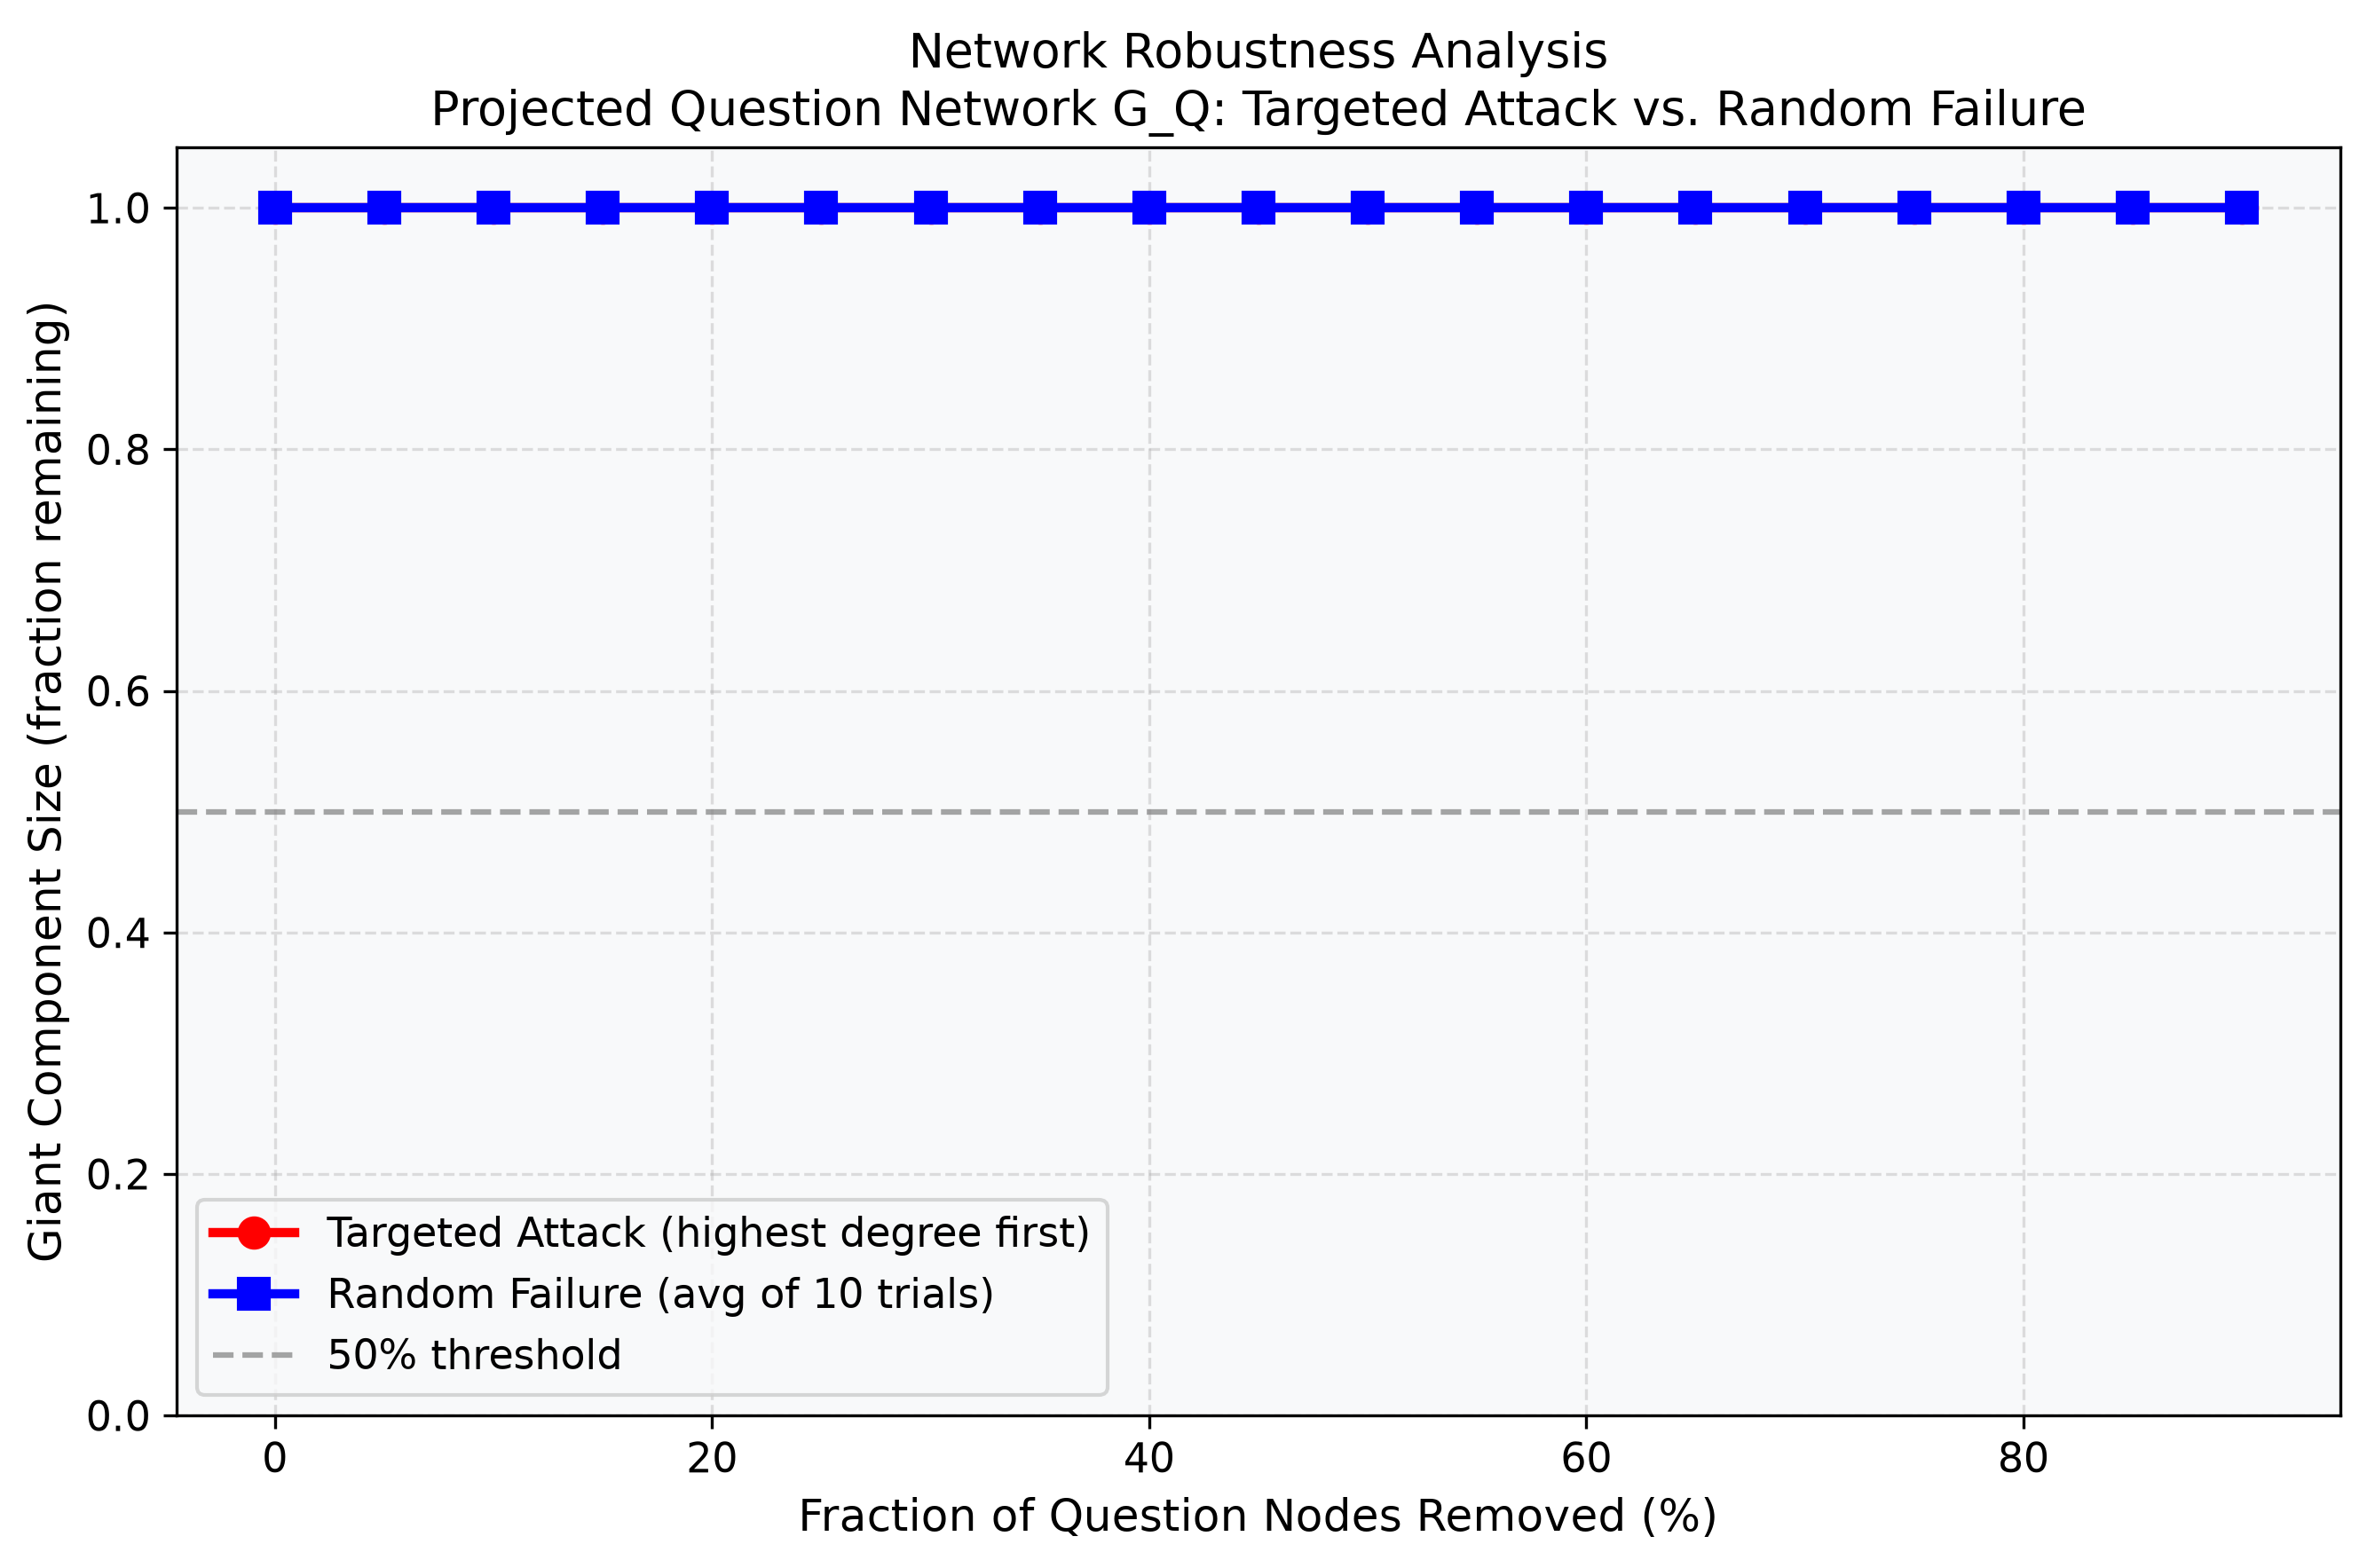
\includegraphics[width=\textwidth]{extreme_plots/robustness_simulation.png}
    \caption{Network robustness analysis: targeted attack (removing highest-degree question nodes first, red) versus random failure (removing randomly selected questions, blue). Because the unweighted projection $G_Q$ is a complete graph ($K_{60}$), the giant component fraction trivially remains a flat line at 1.0 until the network is almost entirely depleted.}
    \label{fig:robustness}
\end{figure}

\subsubsection{The Triviality of Node Removal in $K_{60}$}

As established by the Molloy-Reed parameter ($\kappa = 59.00$), the network is maximally connected. When a robustness simulation is run by removing nodes from the unweighted projection $G_Q$, the result is a flat horizontal line at 1.0 for both random and targeted removals. This occurs because removing a node from a complete graph of size $N$ simply leaves a complete graph of size $N-1$. The giant component remains perfectly intact, demonstrating absolute topological cohesion.

\subsubsection{Indistinguishability of Random Failures and Targeted Attacks}

In a typical scale-free network, a targeted attack on the highest-degree hubs causes a catastrophic collapse of connectivity at very low removal fractions (typically 5--10\%). In our network, however, every question node in the unweighted projection shares the exact same maximal degree of 59. 

Consequently, a "targeted attack" (sorting by highest degree) is mathematically indistinguishable from random failure. There are no topological choke points or single points of failure in the unweighted structure. The extreme-opinion macro-structure is extraordinarily resilient; silencing discussion on a few highly polarizing topics will not fracture the class into isolated echo chambers.

\subsubsection{Comparison: Scale-Free vs. Observed Network}

\begin{center}
\begin{tabular}{lll}
\toprule
\textbf{Property} & \textbf{Scale-Free Network} & \textbf{Observed Network} \\
\midrule
Degree distribution & Power-law $P(k) \propto k^{-\gamma}$ & Bounded, Overdispersed \\
Hub existence & Few dominant mega-hubs & Broad distribution, no mega-hubs \\
Random removal robustness & High (hubs survive) & Absolute ($\kappa = 59 \gg 2$) \\
Targeted attack fragility & Extreme (hub removal $\to$ collapse) & Zero (Targeted = Random) \\
$\kappa = \langle k^2 \rangle / \langle k \rangle$ & Can be $\gg 2$ & 59.000 $\gg 2$ \\
Power-law exponent $\gamma$ & $2 < \gamma < 3$ & $\hat{\gamma} = 0.750$ (not scale-free) \\
Connected components & 1 (giant component) & 1 (complete graph) \\
\bottomrule
\end{tabular}
\end{center}

\subsection{Synthesis: The Ideological Landscape of the Cohort}

Combining all findings, the following coherent picture of the class's ideological landscape emerges:

\textbf{1. The ideological core spans multiple domains.} The top gravity wells are not restricted to a single subject. Instead, Education (E15, E11) and Environment (V13) form the Keystone Trio of hubs. This cohort holds the most intense and polarized views on continuous learning, updating university curricula for emerging tech, and corporate environmental accountability. The presence of highly central questions across all four survey domains proves no single subject monopolizes the ideological core.

\textbf{2. Extreme opinions are a cohesive ideological package.} The completeness of the projected network ($G_Q = K_{60}$) and the single connected component of the raw bipartite graph prove that students with extreme opinions do not form isolated, subject specific factions. A student who holds intense views on education also tends to hold intense views on technology, societal, and environmental questions. Extremism in this cohort is cross cutting and highly integrated.

\textbf{3. The network exhibits absolute topological cohesion.} Because the unweighted projection is a complete graph, the extreme ideological network is extraordinarily resilient. Targeted attacks on polarizing topics are mathematically indistinguishable from random failures. It would take the systematic removal of discussion of nearly all 60 questions to fragment the extreme opinion macrostructure. No single anchor question could isolate a significant faction of students from the broader ideological community if removed from classroom discourse.

\textbf{4. The topology is broad and overdispersed, not elitist.} The bounded degree distribution means that extreme opinions are spread with moderate variance across the question set. This is fundamentally different from a scale free network, where a small number of nodes attract a disproportionate share of connections. In this cohort, while E15 is the most polarizing question, it is not so dramatically more polarizing than average that its removal would fundamentally restructure the network.

\section{Conclusion}

This report constructed and rigorously analyzed a \textbf{Bipartite Extremes Network} mapping the ideological intensity of 96 survey respondents across 60 questions. The five-step pipeline of data preparation, bipartite network construction, degree distribution analysis, centrality computation, and Molloy-Reed evaluation converged on a set of mathematically grounded, empirically verified conclusions:

\begin{enumerate}
    \item \textbf{Primary Anchor:} E15 ("Continuous learning and skill development are essential throughout one's career.") is the single greatest ideological gravity well, attracting extreme views from 71.9\% of the active cohort. The core ideological hubs span multiple domains, led by a Keystone Trio in Education and Environment, reflecting cross-domain ideological intensity.

    \item \textbf{Topology:} The question-node degree distribution is broad and overdispersed, completely lacking a power-law tail ($\hat{\gamma} = 0.750$). This finding definitively rules out a scale-free structure, confirming the absence of disproportional mega-hub questions that monopolize extreme opinion.

    \item \textbf{Complete Projected Graph:} The bipartite projection $G_Q$ is the complete graph $K_{60}$, proving that extreme opinions co-occur across all pairs of questions. No ideological domain silos exist among the highly polarized students.

    \item \textbf{Molloy-Reed:} With $\kappa = \langle k^2 \rangle / \langle k \rangle = 59.000 \gg 2$, the extreme ideological network is maximally percolating. The entire cohort's extreme opinions form one unified, unbroken macro-structure rather than isolated fragmented factions.

    \item \textbf{Structural Robustness:} Because the unweighted projection is a complete graph, the network exhibits absolute topological cohesion. Targeted attacks on polarizing topics are mathematically indistinguishable from random failures, granting the network extraordinary resilience against collapse.
\end{enumerate}

The Bipartite Extremes Network framework, by filtering out all moderate and neutral responses, successfully isolated the most mathematically significant ideological commitments of the cohort and revealed a remarkably coherent, interconnected extreme-opinion landscape.

\end{document}